\documentclass[apj, revtex4-1]{emulateapj}
%\documentclass[apj]{emulateapj}
%%%%% AUTHORS - PLACE YOUR OWN PACKAGES HERE %%%%%
%\usepackage{amsmath}	% Advanced maths commands
%\usepackage{amssymb}	% Extra maths symbols
%\usepackage{mathrsfs}	% Extra extra math symbols

\usepackage{epsf}
\usepackage{color}
\usepackage{amsmath}
\usepackage{graphicx}
\usepackage[colorlinks,urlcolor=magenta,citecolor=blue,linkcolor=blue]{hyperref}
%\usepackage{threeparttable}
%\usepackage{multirow}
\usepackage{natbib}
\usepackage{etoolbox}
\usepackage{longtable}

\bibliographystyle{apj}
\citestyle{aa}

%%%%% AUTHORS - PLACE YOUR OWN COMMANDS HERE %%%%%
%%% Fields %%%
\newcommand{\hdf}{HDF-N}
\newcommand{\hdfn}{HDF-N}
\newcommand{\hdfs}{HDF-S}
\newcommand{\cdfs}{CDF-S}

%%% Telescopes %%%
\newcommand{\hst}{\textit{HST}}
\newcommand{\iras}{\textit{IRAS}}
\newcommand{\iso}{\textit{ISO}}
\newcommand{\spitzer}{\textit{Spitzer}}
\newcommand{\sirtf}{\textit{Spitzer}}
\newcommand{\chandra}{\textit{Chandra}}
\newcommand{\planck}{\textit{Planck}}

%%% Filters %%%
\newcommand{\wfu}{\hbox{$\mathrm{U}_{300}$}}
\newcommand{\wfb}{\hbox{$\mathrm{B}_{450}$}}
\newcommand{\wfv}{\hbox{$\mathrm{V}_{606}$}}
\newcommand{\wfi}{\hbox{$\mathrm{I}_{814}$}}
\newcommand{\acsb}{\hbox{$\mathrm{B}_{435}$}}
\newcommand{\acsv}{\hbox{$\mathrm{V}_{606}$}}
\newcommand{\acsi}{\hbox{$i_{775}$}}
\newcommand{\acsz}{\hbox{$z_{850}$}}
\newcommand{\nicj}{\hbox{$\mathrm{J}_{110}$}}
\newcommand{\nich}{\hbox{$\mathrm{H}_{160}$}}
\newcommand{\wfcy}{\hbox{$\mathrm{Y}_{105}$}}
\newcommand{\wfcj}{\hbox{$\mathrm{J}_{125}$}}
%\newcommand{\wfcj}{\hbox{$J_{110}$}}
\newcommand{\wfch}{\hbox{$\mathrm{H}_{160}$}}
\newcommand{\sdssu}{\hbox{$u$}}
\newcommand{\sdssg}{\hbox{$g$}}
\newcommand{\sdssr}{\hbox{$r$}}
\newcommand{\sdssi}{\hbox{$i$}}
\newcommand{\sdssz}{\hbox{$z$}}
\newcommand{\mone}{\hbox{$[3.6]$}}
\newcommand{\mtwo}{\hbox{$[4.5]$}}
\newcommand{\mthree}{\hbox{$[5.8]$}}
\newcommand{\mfour}{\hbox{$[8.0]$}}
%\newcommand{\mone}{\hbox{$[3.6\mu\mathrm{m}]$}}
%\newcommand{\mtwo}{\hbox{$[4.5\mu\mathrm{m}]$}}
%\newcommand{\mthree}{\hbox{$[5.8\mu\mathrm{m}]$}}
%\newcommand{\mfour}{\hbox{$[8.0\mu\mathrm{m}]$}}

%%% Astronomy Abreviations %%%
\newcommand{\mstar}{\hbox{M$_{\star}$}}
\newcommand{\lstar}{\hbox{L$_{\star}$}}
\newcommand{\Msol}{\hbox{$\mathrm{M}_\odot$}}
\newcommand{\msol}{\hbox{$\mathrm{M}_\odot$}}
\newcommand{\Zsol}{\hbox{$Z_\odot$}}
\newcommand{\zsol}{\hbox{$Z_\odot$}}
\newcommand{\Lsol}{\hbox{$L_\odot$}}
\newcommand{\lsol}{\hbox{$L_\odot$}}
\newcommand{\lir}{\hbox{$L_{\mathrm{IR}}$}}
\newcommand{\zph}{\hbox{$z_\mathrm{ph}$}}
\newcommand{\zphot}{\hbox{$z_\mathrm{ph}$}}
\newcommand{\lbol}{\hbox{$L_\mathrm{bol}$}}
\newcommand{\snr}{\hbox{$\mathrm{S/N}$}}
\newcommand{\reff}{\hbox{$r_\mathrm{eff}$}}
\newcommand{\ks}{\hbox{$K_s$}}
\newcommand{\AAA}{\hbox{\AA}}

%%% Spectrum Lines %%%
\newcommand{\lya}{ Ly$\alpha \;$}
\newcommand{\lyb}{Lyman~$\beta$}
\newcommand{\hb}{\hbox{H$\beta$}}
\newcommand{\ha}{\hbox{H$\alpha$}}
\newcommand{\paa}{\hbox{Pa$\alpha$}}

%%% Units %%%
\newcommand{\kms}{\hbox{km~s$^{-1}$}}
\newcommand{\cms}{\hbox{cm~s$^{-1}$}}
\newcommand{\ergscm}{\hbox{erg~s$^{-1}$~cm$^{-2}$}}
\newcommand{\cnts}{\hbox{cnt~s$^{-1}$}}
\newcommand{\uJy}{\hbox{$\mu$Jy}}
\newcommand{\ujy}{\hbox{$\mu$Jy}}
\newcommand{\degree}{\hbox{$^\circ$}}
\newcommand{\degsq}{\hbox{degree$^2$}}
\newcommand{\arcminsq}{\hbox{arcmin$^2$}}
\newcommand{\um}{\hbox{$\mu$m}}

%%% per Units %%%
\newcommand{\perarcminsq}{\hbox{arcmin$^{-2}$}}
\newcommand{\perdegsq}{\hbox{degree$^{-2}$}}
\newcommand{\permpc}{\hbox{Mpc$^{-1}$}}
\newcommand{\permpcsq}{\hbox{Mpc$^{-2}$}}
\newcommand{\permpccu}{\hbox{Mpc$^{-3}$}}
\newcommand{\percmsq}{\hbox{cm$^{-2}$}}
\newcommand{\percmcu}{\hbox{cm$^{-3}$}}
\newcommand{\perpixel}{\hbox{pixel$^{-1}$}}

%%% Math %%%
\newcommand{\lsim}{\lesssim}
\newcommand{\gsim}{\gtrsim}
\newcommand{\mathS}{\hbox{$\mathcal{S}$}}
\newcommand{\mathR}{\hbox{$\mathcal{R}$}}
\newcommand{\mathM}{\hbox{$\mathcal{M}$}}
\newcommand{\mcal}{\hbox{$\mathcal{M}$}}
\newcommand{\rcal}{\hbox{$\mathcal{R}$}}
\newcommand{\scal}{\hbox{$\mathcal{S}$}}
\newcommand{\infinity}{\hbox{$\infty$}}
\newcommand{\err}[2]{$^{+#2}_{-#1}$}

%%% General %%%
\newcommand{\etal}{et al.}
\newcommand{\eg}{e.g.}
\newcommand{\ie}{i.e.}
\newcommand{\cf}{cf.}
% \newcommand{\ion}[2]{\hbox{#1$\;${\small\rm{#2}}}}
\newcommand{\mybullet}{\noindent$\bullet$}
\newcommand{\uit}{\textit{UIT}}
\newcommand{\nd}{...}
%\newcommand{\cmodel}{\hbox{\tt cmodel}}
%\newcommand{\bs}{\hbox{$\!\!\!\!$}}
\newcommand{\todo}[1]{{\tt #1}}
\newcommand{\citeeg}[1]{(\eg, \citealt{#1})}
\newcommand{\ignore}[1]{}

%%% Extra %%%
% \newcommand{\farcm}{\mbox{\ensuremath{.\mkern-4mu^\prime}}}    % fractional arcminute symbol: 0.'0
% \newcommand{\farcs}{\mbox{\ensuremath{.\!\!^{\prime\prime}}}}  % fractional arcsecond symbol: 0.''0
% \newcommand{\fdg}{\mbox{\ensuremath{.\!\!^\circ}}}             % fractional degree symbol:    0.°0
%\newcommand{\arcdeg}{\ensuremath{^{\circ}}}%                    % degree symbol:  °
% \newcommand{\sun}{\ensuremath{\odot}}%                         % sun symbol
% \newcommand{\apj}{ApJ}%                                        % Journal abbreviations
% \newcommand{\apjs}{ApJS}
% \newcommand{\apjl}{ApJL}
% \newcommand{\aap}{A{\&}A}
% \newcommand{\aaps}{A{\&}AS}
% \newcommand{\mnras}{MNRAS}
% \newcommand{\aj}{AJ}
% \newcommand{\araa}{ARAA}
% \newcommand{\pasp}{PASP}
\newcommand{\Teff}{\ensuremath{T_{\mathrm{eff}}}}%               % T_eff
\newcommand{\logg}{\ensuremath{\log g}}%                         % log g
%\newcommand{\bv}{\ensuremath{B\!-\!V}}%                         % B-V
%\newcommand{\ub}{\ensuremath{U\!-\!B}}%                         % U-B
%\newcommand{\vr}{\ensuremath{V\!-\!R}}%                         % V-R
%\newcommand{\ur}{\ensuremath{U\!-\!R}}%                         % U-R
%\newcommand\ion[2]{#1$\;${\scshape{#2}}}%                       % ion, i.e., CII = \ion{C}{ii}


\newcommand{\editorial}[1]{\textcolor{red}{#1}}
\newcommand{\peditorial}[1]{\textcolor{blue}{#1}}
\newcommand{\multic}[2]{\multicolumn{#1}{c}{#2}}
\newcommand{\rottext}[2]{\multirow{#1}{*}{\rotatebox[origin=c]{90}{#2}}}

\makeatletter
% Patch case where name and year are separated by aysep
\patchcmd{\NAT@citex}
{\@citea\NAT@hyper@{%
		\NAT@nmfmt{\NAT@nm}%
		\hyper@natlinkbreak{\NAT@aysep\NAT@spacechar}{\@citeb\@extra@b@citeb}%
		\NAT@date}}
{\@citea\NAT@nmfmt{\NAT@nm}%
	\NAT@aysep\NAT@spacechar\NAT@hyper@{\NAT@date}}{}{}

% Patch case where name and year are separated by opening bracket
\patchcmd{\NAT@citex}
{\@citea\NAT@hyper@{%
		\NAT@nmfmt{\NAT@nm}%
		\hyper@natlinkbreak{\NAT@spacechar\NAT@@open\if*#1*\else#1\NAT@spacechar\fi}%
		{\@citeb\@extra@b@citeb}%
		\NAT@date}}
{\@citea\NAT@nmfmt{\NAT@nm}%
	\NAT@spacechar\NAT@@open\if*#1*\else#1\NAT@spacechar\fi\NAT@hyper@{\NAT@date}}

%%%%%%%%%%%%%%%%%%% TITLE PAGE %%%%%%%%%%%%%%%%%%%
 %-----------------------------------------------------------------------------------------

\shorttitle{}
\shortauthors{BOADA ET AL.}

\slugcomment{\it Draft Version \today}
%\slugcomment{\it Submitted for publication in the Astrophysical Journal}
%\slugcomment{Accepted for Publication in the Astrophysical Journal}

\begin{document}

\title{Planck Cluster Paper}

\author{\sc Steven Boada\altaffilmark{1},
John P. Hughes\altaffilmark{1},
Felipe Menanteau\altaffilmark{2,3},
Peter Doze\altaffilmark{1},
L. Felipe Barrientos\altaffilmark{4},
L. Infante\altaffilmark{4}
}

\altaffiltext{1}{Department of Physics and Astronomy, Rutgers, the State University of New Jersey, 136 Frelinghuysen Road, Piscataway, NJ 08854-8019, USA; \href{mailto:boada@physics.rutgers.edu}{boada@physics.rutgers.edu}}
\altaffiltext{2}{National Center for Supercomputing Applications, 1205 West Clark St., Urbana, IL 61801, USA}
\altaffiltext{3}{Department of Astronomy, University of Illinois at Urbana-Champaign, 1002 W. Green Street, Urbana, IL 61801, USA}
\altaffiltext{4}{Instituto de Astrof\'isica y Centro de Astroingeniería, Facultad de Física, Pontificia Universidad Cat\'olica de Chile, Casilla 306, Santiago 22, Chile}


\begin{abstract}
\noindent We report on newly identified galaxy clusters selected from the second all-sky \planck\ Sunyaev-Zel'dovich (SZ) catalog (PSZ2), and have a detection of at least $5\sigma$. The clusters are identified in optical imaging from the Kitt Peak National Observatory 4m Mayall telescope taken between 2014 and 2017. Focusing on the highest richness systems, we identify galaxy clusters through a combination of the maxBCG algorithm and visual image inspection. Galaxy clusters are considered to be confirmed if they are both rich (Ngal $>20$) and spatially coordinate ($<5'$) with the reported PSZ2 position. Of the 85 fields containing unconfirmed sources observed, we characterize 18 (21\% of observed sample) correspondent galaxy clusters ($ 0.13 < z < 0.74$), 15 of which are previously unknown. We discuss three possible scenarios -- all low-$z$, all high-$z$, obscured by the Milky Way -- which could lead to the low identification fraction, and determine that no single scenario could account for the low purity of rich galaxy clusters.
\end{abstract}

\section{Introduction}
Galaxy clusters, especially massive clusters, are extraordinary objects which contain vital clues to the structure and evolution of the universe. The generally accepted $\Lambda$CDM cosmological model makes detailed predictions about the number and total mass distribution of galaxy clusters throughout the universe. These galaxy clusters, particularly at high redshift, play a cruicial role in constraining large scale structure formation and evolution \citeeg{Mortonson2011, Harrison2012, Harrison2013, Waizmann2013}.

Large-area sky surveys, both currently underway and planned, are identifying many tens of thousands of galaxy clusters for both detailed examinations of our cosmological models and as probes of fundamental physics. Today, the largest number of galaxy clusters are identified through ground based, millimeter wave surveys conducted by the South Pole Telescope (SPT; \citealt{Carlstrom2011} or the Atacama Cosmology Telescope (ACT; \citealt{Swetz2011}), among others. These surveys have identified hundreds of massive galaxy clusters below $z \sim 1.4$ \citeeg{Brodwin2010, Foley2011, Menanteau2012, Hasselfield2013a, Reichardt2013, Bayliss2016}. This detection approach exploits the cluster's hot intracluster medium which imprints a telltale signature on the Cosmic Microwave Background (CMB) through the Sunyaev-Zel'dovich effect (SZ; \citealt{Sunyaev1972}) effect.

Deep, wide field photometric surveys such as the ongoing Hyper Suprime-Cam Survey \citep{Aihara2018a} and Dark Energy Survey (DES; \citealt{DES2005}), as well as future surveys like the Large Synoptic Survey Telescope (LSST; \citealt{LSST2012}), \textit{Euclid}, and WFIRST will discover many thousands additional galaxy clusters at redshifts to $z=1$ \citeeg{DarkEnergySurveyCollaboration2016} and beyond. While a powerful discovery method, photometric surveys suffer from cosmological dimming or K-correction \citep{Hogg2002}. \editorial{Need more words.}

Using the SZ effect to discover clusters of galaxies has the distinct advantage that the surface brightness of the SZ effect does not dim with increasing redshift. This allows homogeneous samples of massive clusters to be detected out to arbitrary distances. Now, \planck\ \citep{Tauber2010, PlanckCollaboration2011} has released an all-sky SZ sample (hereafter PSZ; \citealt{PlanckCollaboration2014, PlanckCollaboration2015a}) that contains 1943 detections with 1330 confirmed clusters and another 613 (currently) unconfirmed cluster candidates. Clusters were initially confirmed by cross correlating with previous catalogs (see Section 4; \citealt{PlanckCollaboration2014}). More recently, dedicated follow up of still-unconfirmed clusters has begun in earnest \citeeg{Liu2015a, PlanckCollaboration2015, PlanckCollaboration2016a, VanderBurg2016, Burenin2017, Barrena2018, Amodeo2018, Streblyanska2018}.

In this paper we report on our efforts to classify unconfirmed PSZ sources. This paper is organized as follows: sections \ref{sec:design} through \ref{sec:analysis} describe the design, observations, data reduction and calibration, and creation of derived data products. In Section~\ref{sec:results}, we present the main results of our observations, and discuss the results in Section~\ref{sec:discussion}. In Section~\ref{sec:summary}, we summarize the key results and conclude.

Unless otherwise noted, throughout this paper, we use a concordance cosmological model ($\Omega_\Lambda = 0.7$, $\Omega_m = 0.3$, and $H_0= 70$ \kms \permpc), assume a Chabrier initial mass function \citep{Chabrier2003}, and use AB magnitudes \citep{Oke1974}.

\section{Design}\label{sec:design}
Our observational design is motivated by the release of the second, all-sky PSZ catalog\footnote{\url{http://szcluster-db.ias.u-psud.fr/sitools/client-user/SZCLUSTER_DATABASE/project-index.html}} (hereafter PSZ2; \citealt{PlanckCollaboration2015a}) which contains 559 unconfirmed SZ detections with signal-to-noise ratio (SNR) $> 4.5$. We posit that the vast majority of these must lie at $z>0.4$ because the \planck\ confirmation process \citep{PlanckCollaboration2014} mostly relied on existing catalogs which have a preference for low$-z$ clusters. Furthermore, the confirmed sample of PSZ2 has only a small fraction (3\%) of $z > 0.6$ clusters compared to that expected ($\sim20$\%) based on the theoretical halo mass function \citeeg{Jenkins2001, Tinker2008} for mass limit of $6\times10^{14}$ \msol. If other clusters as massive like el ``El Gordo'' exist, they are hiding as high-significance candidates within the objects in this \textit{it all-sky} catalog.

The core of our observational design relies on the use of optical imaging to confirm the SZ detections as real clusters and provide photometric redshifts using the multi-color information. This design is based on the previous success with the ACT cluster confirmation process using 4-m class telescopes.
%
For example, assuming WMAP7 cosmology \citep{Komatsu2011} with the \cite{Tinker2008} halo mass function, there should be only $\sim4$ clusters as massive as ``El Gordo'' ($\leq 2 \times 10^{15}$ \Msol) at $z > 0.6$ in the full area covered by the \planck\ PSZ catalog (83.7\% of the sky). Although \planck’s larger beam size (compared to both ACT and SPT) makes it more sensitive to clusters at lower redshifts (due to their larger projected area on the sky), among the confirmed clusters in the recently released all-sky \planck\ SZ catalog are the two highest significance high-redshift SZ detections from ACT (as well as several other ACT and SPT clusters).

Our strategy for this project is to use the Kitt Peak National Observatory (KPNO) Mayall-4m telescope imaging as the first and fundamental step to confirm the highest significance detections in the PSZ2 catalog that are visible across the entire northern sky.
%
%We initially focus on the northern sky as we anticipate the release of
%the Dark Energy Survey (DES; \citealt{DES2005}) Data Release 1 (DR1;
%\citealt{Abbott2018}) imaging and catalogs.
%
Following closely the procedure used for ACT follow-up \citeeg{Menanteau2013}, targets are prioritized by SZ SNR. We choose to initially report on targets with PSZ2 SNR $>5$ as the statistical reliability of PSZ2 cluster candidates should be quite high: according to the \planck\ team $\sim90$\% of candidates at SNR $>5$ are expected be ``real'' clusters (see Figure 11; \citealt{PlanckCollaboration2015a}).
%
Optical imaging should be sufficient to confirm nearly all of the candidates, but for the highest redshift ones, near-IR data will be necessary. Again following the procedure for ACT cluster follow-up: those candidates with some evidence for a high$-z$ brightest cluster galaxy (BCG) will be targeted with near-IR observations to confirm the presence of a BCG and detect the red sequence of cluster members. Observational priority again is given to higher SNR candidates.

\subsection{Observations}\label{sec: observations}
All observations were conducted with the KPNO Mayall telescope. The optical observations were made with the MOSAIC camera mounted at the prime focus. Two detector packages were used for the observations. The earlier MOSAIC1.1 instrument consisted of eight $2048\times4096$ SITe CCDs, arranged $2\times4$, separated by a $∼\sim50$ pixels gap with a pixel scale of $0\farcs26$ \perpixel. MOSAIC1.1 was replaced with MOSAIC3, in mid-2015, and consists of four new 4k$\times$4k, 15 micron pixel, 500-micron thick LBNL deep-depletion CCDs. Because the only change from MOSAIC1.1 to MOSAIC3 are the CCDs and controllers both versions have a $36' \times 36'$ field-of-view.

The optical observing strategy consists of targeted $griz$ observations of individual candidates with total exposure times of 360 s, 360 s, 1100 s and 1100 s (assuming dark conditions). The final exposures consist of four dithered positions with individual exposures of 90 s for the $gr$-bands or 275 s for the $iz$-bands. These exposure times are designed to ensuring the unambiguous detection of the faint galaxies in the red cluster sequence up to $z \sim 1.0$ \editorial{(citation?)} and of brightest cluster galaxies (BCGs) to higher redshifts. The choice of filters in our program is driven by the need to segregate early-type galaxies in the cluster through their colors (or photometric redshifts) by sampling blue-ward and red-ward of the 4000\AA\ break.

\section{Data Reduction and Calibration}\label{sec:data reduction}
Standard image reductions including subtraction of dark frames, flat fielding, sky-subtraction, and bad pixel masking was performed by the NOAO virtual observatory using the MOSAIC \citep{Valdes2007} science pipelines. The resultant FITS files consist of fully reduced images with either all single exposure CCDs mosaicked into a single image extension (as in the case of Mosaic1.1) or as a multi-extension FITS file with each single exposure CCD occupying a separate extension.

We then mosaic each separate exposure into a master mosaic as described in the following section.

\subsection{Mosaicking}\label{sec:mosaicks}
Combined mosaics are created with \textsc{swarp} \citep{Bertin2002}. We create three distinct types of mosaics. The individual dither frames are stacked and then median combined to produce the final completed science mosaic. A ``detection'' is created by combining select science mosaics into a ``chi2'' image using either the \sdssi- and \sdssz-band when both are available and of sufficient quality. Finally we create a set of mosaics use to produce the three color image used for cluster finding. We median combine the \sdssg\sdssr\sdssi\sdssz\ science mosaics into a ``blue'' (\sdssg-band), ``green'' (\sdssr-band), and ``red'' (\sdssi\sdssz-band) mosaic. All final mosaics have a pixel scale of $0\farcs25$ \perpixel. The final exposure time is calculated as the median exposure time of the combined images, and similarly the final airmass is median of the individual air masses.

%The full parameter file used while creating the mosaics is given in Appendix~\ref{app:swarp}.

\subsection{Source Extraction and Photometry}\label{sec:sextractor}
For source extraction and photometry estimation we use Source Extractor (hereafter SExtractor; version $2.19.5$; \citealt{Bertin1996}) run dual image mode with the CHI2 detection image as the detection image. See Section~\ref{sec:mosaicks}.

%See Appendix~\ref{app:sextractor} for a complete parameter listing.

\subsection{Astrometric Calibration}
Each of the final science mosaics produced in the previous section are first astrometrically aligned with \textit{Gaia} \citep{GaiaCollaboration2016} Data Release 1 \citep{GaiaCollaboration2016a} using \textsc{scamp} \citep{Bertin2006} as a part of \textsc{photometrypipeline}\footnote{\url{https://github.com/mommermi/photometrypipeline}} (PP; \citealt{Mommert2017}).

Sources are extracted from the mosaics with a SNR of at least ten and with a minimum area of at least 12 pixels. The extracted sources are then matched to the \textit{Gaia} data and a new astrometric solution is calculated. Matching all science images to the \textit{Gaia} world coordinate system ensures that we have a common alignment across all observing runs. Because the initial astrometric solution from the VO is quite accurate, the resultant corrections are much less than $1''$.

\subsection{Photometric Calibration}
After the mosaics have been astrometrically aligned, we use PP to produce a photometric solution. PP calculates a photometric zero-point in each of our observed bands by comparing field stars located throughout the science mosaic to known photometry from large-area sky surveys. Because our sources are spread across the entire northern sky, and because we prefer to minimize the number of differences between photometric solutions we are limited to two optical surveys. We first seek photometric data from the \textit{Sloan Digital Sky Survey} (SDSS; \citealt{York2000}) Data Release 13 (DR13; \citealt{Albareti2017}). When our target does not lie within the SDSS footprint we utilize the Panoramic Survey Telescope and Rapid Response System (Pan-STARRS; \citealt{Chambers2016}) Data Release 1 (hereafter PS1; \citealt{Flewelling2016}). Both surveys provide accurate \sdssg\sdssr\sdssi\sdssz\ magnitudes and large on-line queriable databases for rapid automated calibration.

Sources are extracted from the combined mosaics with either a $3''$ (12 pixel) diameter aperture for optical sources respectively; sources with a SNR $\ge10$ are matched to a survey catalog and a photometric zero-point is determined. We use half of the available stars (with accurate catalog photometry) to derive the zero-point resulting in zero-points calculated from approximately $10-500$ stars and with typical uncertainties of 0.05 mag for the \sdssg\sdssr\sdssi-bands and 0.16 mag for the \sdssz-band.

\section{Analysis}\label{sec:analysis}
\subsection{Photometric Redshifts}
\editorial{Try to clean up the use of ``photo-z'' vs. $z_\mathrm{phot}$ vs. $z_\mathrm{bpz}$ and all of that stuff to make sure we are consistent}
We determine photometric redshifts (photo-$z$) from the five-band optical images using Bayesian Photometric Redshifts (BPZ; \citealt{Benitez2000, Coe2006}) following the same procedure as in \cite{Menanteau2009a}.

We assess the effectiveness of our photo-$z$ estimates by comparing with the available spectroscopic redshifts (spec$-z$) from the SDSS. We use three diagnostics to gauge photo-$z$ accuracy. First, we report the full scatter between the photo-$z$ and spec-$z$, defined as:
\begin{equation}\label{eqn:scatter}
	\sigma_f = \mathrm{RMS}[\delta z/(1+z_\mathrm{spec})]
\end{equation}
where $\delta z = z_\mathrm{spec} - z_\mathrm{phot}$. Second, we report the normalized median absolute deviation (NMAD; \citealt{Ilbert2009, Dahlen2013, Molino2017}), given as
\begin{equation}\label{eqn:nmad}
	\sigma_\mathrm{NMAD} = 1.48 \times \mathrm{median} \bigg{(} \frac{|\delta z|}{1+z_\mathrm{spec}} \bigg{)}.
\end{equation}
which provides an estimate of the scatter resistant to catastrophic outliers. Finally, the catastrophic outlier fraction (OLF) where we define a catastrophic outlier (following \citealt{Molino2017}) as,
\begin{equation}\label{eqn:OLF}
	\eta = \frac{|\delta z|}{(1+z_\mathrm{spec})} > 5 \times \sigma_\mathrm{NMAD}.
\end{equation}

\begin{figure}
	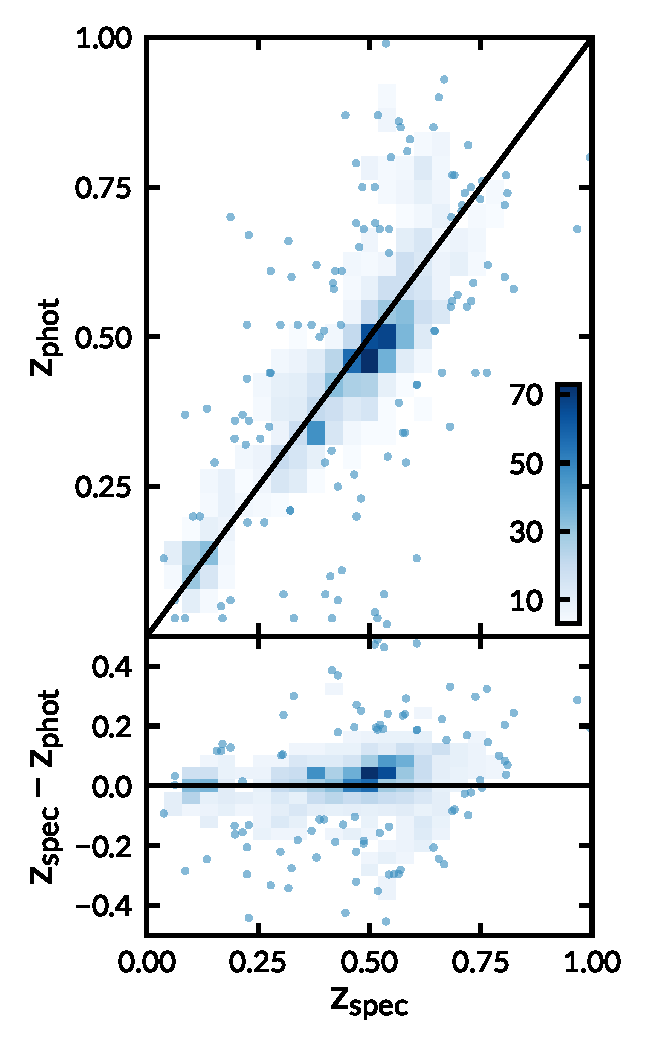
\includegraphics[width=\columnwidth]{figures/specVSphot.pdf}
	\caption{Comparison between photometric and spectroscopic redshifts for 1588 elliptical galaxies which have spectroscopic redshifts from the SDSS. \textit{Top:} The photometric redshifts are those reported by BPZ with a custom empirical prior on galaxy brightness for the photometric redshifts. \textit{Bottom:} The difference between the spectroscopic and photometric redshifts, $z_\mathrm{spec} - z_\mathrm{bpz}$, as a function of spectroscopic redshift. In both panels the shading scales (darker is greater) with the density of points where bins with fewer than three points are shown as single points. The solid black line shows the 1:1 relation.}
	\label{fig:photozspecz}
\end{figure}

Figure~\ref{fig:photozspecz} shows the photo-$z$ performance as a function of the true spectroscopic redshift. Because we are primarily concerned with identifying clusters containing early-type galaxies galaxies, we show only galaxies classified E/S0 by BPZ. We find $\sigma_f = 0.067$, $\sigma_\mathrm{NMAD} = 0.048$, and an outlier fraction, $\eta = 0.9\%$.

\subsection{Cluster Finding}
In this section, we briefly describe the algorithms and methods use to select the galaxy clusters from the multi-wavelength optical imaging. We follow the methods described in detail in \cite{Menanteau2009a, Menanteau2010} and direct the reader there for an in depth description and discussion of the methods.

We first create a three-color image using \textsc{stiff} \citep{Bertin2011}. The red, green, and blue channels are given by the corresponding combined mosaics described in Section~\ref{sec:mosaicks}. We then visually inspect an area of roughly $8' \times 8'$ centered on the position of each unconfirmed PSZ detection. Potential BCGs are selected manually, and are identified by their characteristic colors and accompanying member galaxies.

% more words describing what the algorithm does?

Once a potential BCG is selected, the algorithm selects nearby galaxies, within $|z_\mathrm{BCG} - z| < 0.05$ and 0.5 Mpc projected radius, which BPZ has classified as either E or E/S0 galaxies. These photo-$z$'s of the galaxies are combined using a $3\sigma$ median sigma-clipping algorithm to estimate the cluster's mean redshift, $z_c$. We use this mean cluster redshift measurement and the member selection criteria given previously to estimate the number of cluster members within 1 Mpc, $N_\mathrm{1 Mpc}$, which we define as the richness \citeeg{Abell1958} of the cluster, $N_\mathrm{gal}$.

We correct the $N_\mathrm{gal}$ estimate by subtracting a statistical background of galaxies. We first estimate the number of background ellipticals by selecting galaxies within an annulus ($R_{200} <r < 2R_{200}$) around each cluster's position. We include galaxies with $\delta z = 0.05$ and similar colors as those galaxies assumed to belong to the cluster. These galaxies are subtracted from the cluster's population which provides an corrected $N_\mathrm{gal}$, $N_\mathrm{galc}$, which we then use to compute other important quantities. In practice the corrected number of galaxies is between 15\% and 20\% lower than the uncorrected number \citep{Menanteau2010}. We report $N_\mathrm{galc}$ for the remainder of this work.

\subsection{Recovery of the Brightest Cluster Galaxies}\label{sec:cluster finding}
We have designed our observations to detect BCGs to $z\sim1.5$. To quantify the actual depths of our images, we perform two distinct tests. First, we perform a Monte Carlo simulation by injecting artificial sources and compute their recovery fractions. Second, we fit a power-law model to the bright side of each field's dn/dm curve and identify the magnitude at which dn/dm is a specific fraction of the model.

The Monte Carlo simulation broadly follows the procedure given in \cite{Menanteau2010a}. We create the artificial sources with the \textsc{modeling} package, part of \textsc{astropy} \citep{TheAstropyCollaboration2013}. The synthetic galaxies are created to have de Vaucouleurs \citep{DeVaucouleurs1948} profiles and surface brightnesses corresponding to their magnitude and assumed sizes. We inject the artificial galaxies into our science images with similar noise characteristics as their real counterparts.

We generate ten rounds of one hundred elliptical galaxies spread randomly across our science imaging. Each round of galaxies are placed at different random positions to suppress abnormally boosted recovery fractions due to source confusion. The artificial galaxies have total fluxes corresponding to apparent magnitudes between 20 mag $< \sdssi <$ 25 mag with $0.2$ mag spacing. We report the 80\% \sdssi-band limit for each field, which is the magnitude where 80\% of the simulated galaxies are recovered.

\begin{figure*}
	\centering
	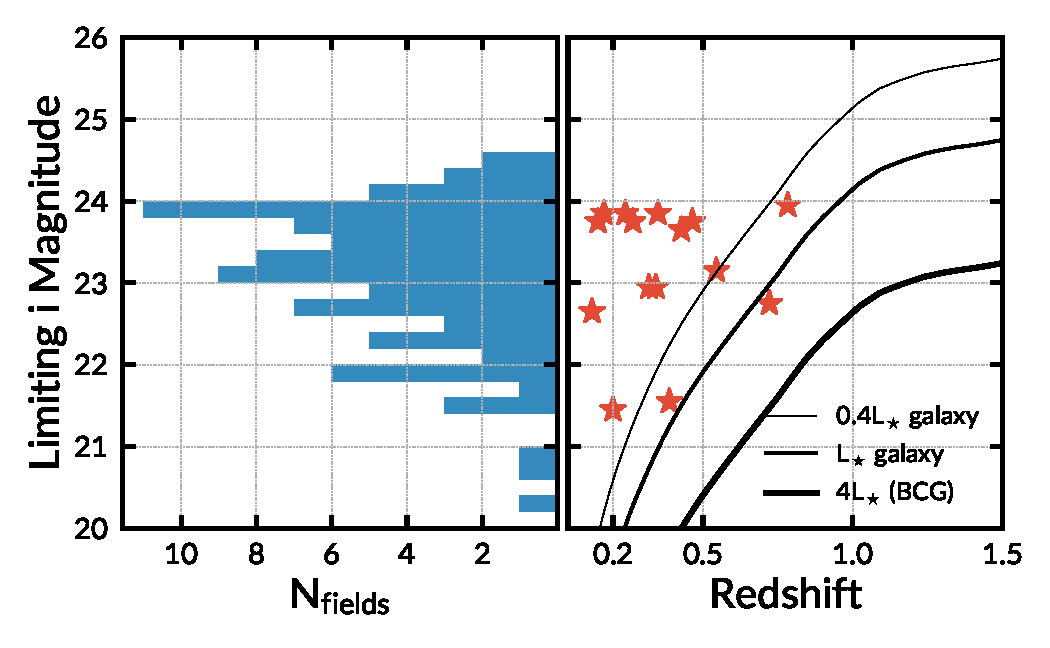
\includegraphics[width=0.8\textwidth]{figures/recovery_redshift.pdf}
	\caption{\textit{Left:} Histogram of the \sdssi-band magnitude corresponding to 80\% completeness in galaxy recovery. When 80\% completeness is not achieved we show the limiting magnitude with the highest completeness. \textit{Right:} Observed \sdssi-band magnitudes of $\lstar$, $0.4\lstar$, and $4\lstar$ (BCG) early-type galaxies as a function of redshift. We define an \lstar\ galaxy following \cite{Blanton2003} as a population of red galaxies at $z = 0.1$ and allow it to evolve passively. The left and right panels can be combined to estimate the limiting redshift to which we could identify galaxy clusters.}
	\label{fig:recovery_redshift}
\end{figure*}

The second method to estimate the limiting magnitudes of our observations uses the calibrated SExtractor catalogs (see Section~\ref{sec:sextractor}). We bin the objects identified by SExtractor as galaxies in 0.5 mag wide bins from $15<$ \sdssi\ $<30$. We identify the peak of the dn/dm curve in log space and fit a power-law model to the five bins on the bright side of the peak. The 80\% completeness limit is defined as the magnitude bin at which the value of dn/dm is 80\% of the expected model value.

The completeness limits reported by each method are consistent and provide an important check on one another as they are wholly independent estimates of the limiting \sdssi-band magnitude in each of our fields. We choose to focus on the limiting magnitudes reported by the power-law based method as it is less prone to errors from very bright stars or diffuse emission from the Milky Way also present in the field.

With a limiting magnitude reported for each field, we are able to estimate the redshift to which we could reliably identify massive galaxy clusters. We compare the completeness limits of our observations to the expected (\ie, known) apparent magnitudes of galaxies in clusters as a function of redshift. We define the expected apparent \sdssi-band magnitude of a galaxy following the population of red galaxies defined by \cite{Blanton2003}. The \lstar, 0.4\lstar, and 4\lstar galaxies (representing faint members to bright BCGs) are composed of stars formed in a burst at $zf = 5$, with solar metallicity \citep{Bruzual2003}, and allowed to evolve passively, $\tau = 1.0$ Gyr. We show the expected \sdssi-band apparent magnitude as a function of redshift for each galaxy in the right panel of Figure~\ref{fig:recovery_redshift}.

\section{Results}\label{sec:results}
In this section, we give the results of our cluster finding. We report high confidence, high richness clusters. A high confidence result consists of a clear BCG and many accompanying satellite galaxies. For the 85 fields observed with MOSAIC, we observe fifteen high confidence clusters (see Figures~\ref{fig:Clusters1}--\ref{fig:Clusters4}). In the following subsections we present on each of the eight high confidence observations individually, and group the medium and low confidence observations together.

\begin{figure*}
	\centering
	\begin{tabular}{cc}
		\includegraphics[width=0.47\linewidth]{figures/{PSZ2_G029.66-47.63}.pdf}&
		\includegraphics[width=0.47\linewidth]{figures/{PSZ2_G043.44-41.27}.pdf}\\
		\includegraphics[width=0.47\linewidth]{figures/{PSZ2_G084.62-15.86}.pdf}&
		\includegraphics[width=0.47\linewidth]{figures/{PSZ2_G096.43-20.89}.pdf}
	\end{tabular}
	\caption{RGB (\sdssi\sdssr\sdssg) color images for four PSZ clusters optically confirmed using the our optical imaging. Each panel is centered on the cluster's BCG and has a width of 1 mpc at the corresponding cluster's redshift. The horizontal bar in the lower left of each panel shows the scale of the panel, where north is up and east is to the left. The location of the PSZ detection is denoted by a red star. The dashed and solid concentric circles are $2'$ and $5'$ in radius respectively.}
	\label{fig:Clusters1}
\end{figure*}

\begin{figure*}
	\centering
	\begin{tabular}{cc}
		\includegraphics[width=0.47\linewidth]{figures/{PSZ2_G098.38+77.22}.pdf}&
		\includegraphics[width=0.47\linewidth]{figures/{PSZ2_G106.11+24.11}.pdf}\\
		\includegraphics[width=0.47\linewidth]{figures/{PSZ2_G107.83-45.45}.pdf}&
		\includegraphics[width=0.47\linewidth]{figures/{PSZ2_G120.76+44.14}.pdf}
	\end{tabular}
	\caption{RGB (\sdssi\sdssr\sdssg) color images for four PSZ clusters optically confirmed using the our optical imaging. Each panel is centered on the cluster's BCG and has a width of 1 mpc at the corresponding cluster's redshift. The horizontal bar in the lower left of each panel shows the scale of the panel, where north is up and east is to the left. The location of the PSZ detection is denoted by a red star. The dashed and solid concentric circles are $2'$ and $5'$ in radius respectively.}
	\label{fig:Clusters2}
\end{figure*}

\begin{figure*}
	\centering
	\begin{tabular}{cc}
		\includegraphics[width=0.47\linewidth]{figures/{PSZ2_G125.55+32.72}.pdf}&
		\includegraphics[width=0.47\linewidth]{figures/{PSZ2_G137.24+53.93}.pdf}\\
		\includegraphics[width=0.47\linewidth]{figures/{PSZ2_G173.76+22.92}.pdf}&
		\includegraphics[width=0.47\linewidth]{figures/{PSZ2_G191.82-26.64}.pdf}
	\end{tabular}
	\caption{RGB (\sdssi\sdssr\sdssg) color images for four PSZ clusters optically confirmed using the our optical imaging. Each panel is centered on the cluster's BCG and has a width of 1 mpc at the corresponding cluster's redshift. The horizontal bar in the lower left of each panel shows the scale of the panel, where north is up and east is to the left. The location of the PSZ detection is denoted by a red star. The dashed and solid concentric circles are $2'$ and $5'$ in radius respectively.}
	\label{fig:Clusters3}
\end{figure*}

\begin{figure*}
	\centering
	\begin{tabular}{cc}
		\includegraphics[width=0.47\linewidth]{figures/{PSZ2_G206.45+13.89}.pdf}&
		\includegraphics[width=0.47\linewidth]{figures/{PSZ2_G224.82+13.62}.pdf}\\
		\includegraphics[width=0.47\linewidth]{figures/{PSZ2_G305.76+44.79}.pdf}&
	\end{tabular}
	\caption{RGB (\sdssi\sdssr\sdssg) color images for four PSZ clusters optically confirmed using the our optical imaging. Each panel is centered on the cluster's BCG and has a width of 1 mpc at the corresponding cluster's redshift. The horizontal bar in the lower left of each panel shows the scale of the panel, where north is up and east is to the left. The location of the PSZ detection is denoted by a red star. The dashed and solid concentric circles are $2'$ and $5'$ in radius respectively.}
	\label{fig:Clusters4}
\end{figure*}

\begin{table*}
	\caption[Summary of Cluster Finding]{Summary of cluster finding: Column 1: The PSZ2 cluster name; Column 2: PSZ2 signal-to-noise ratio; Column 3: PSZ1 ID number; Column 4: BCG Right Ascension in J2000; Column 5: BCG Declination in J2000; Column 6: BCG separation from PSZ position in arcmintues; Column 7: Cluster photometric redshift with 1-$\sigma$ uncertanty; Column 8: Corrected number of member galaxies; Column 9: New confirmation? }
	\centering
	\begin{tabular}{lcccccccc}
	\hline
	Cluster & SNR & PSZ1 ID & $\alpha$ (J2000) & $\delta$ (J2000) & Sep. ($'$) & $z_\mathrm{cl}$ & Ngal$_c$ & New\\
	(1) & (2) & (3) & (4) & (5) & (6) & (7) & (8) & (9) \\
	\hline
	 PSZ2 G$029.66-47.63$ & 5.74 & \nd & $21:45:29.940$ & $-21:43:26.29$ & 4.73 & $0.34 \pm 0.03$ & 130 & $\checkmark$ \\
	 PSZ2 G$043.44-41.27$ & 5.55 & \nd & $21:36:43.728$ & $-10:19:02.15$ & 1.24 & $0.42 \pm 0.04$ & 116 & $\checkmark$ \\
	 PSZ2 G$084.62-15.86$ & 6.01 & 284 & $21:49:42.524$ & $+33:09:17.29$ & 1.14 & $0.27 \pm 0.10$ & 18 & \\
	 PSZ2 G$096.43-20.89$ & 5.81 & \nd & $22:48:09.402$ & $+35:33:49.45$ & 0.49 & $0.24 \pm 0.04$ & 54 & $\checkmark$ \\
	 PSZ2 G$098.38+77.22$ & 5.51 & 346 & $13:18:08.274$ & $+38:30:20.10$ & 5.84 & $0.78 \pm 0.05$ & 58 & $\checkmark$ \\
	 PSZ2 G$106.11+24.11$ & 5.70 & \nd & $19:21:31.852$ & $+74:33:27.17$ & 0.51 & $0.14 \pm 0.06$ & 27 & $\checkmark$ \\
	 PSZ2 G$107.83-45.45$ & 7.09 & \nd & $00:07:35.605$ & $+16:07:02.39$ & 0.83 & $0.54 \pm 0.05$ & 30 & $\checkmark$ \\
	 PSZ2 G$120.76+44.14$ & 5.59 & \nd & $13:12:53.537$ & $+72:55:06.05$ & 2.02 & $0.35 \pm 0.03$ & 92 & $\checkmark$ \\
	 PSZ2 G$125.55+32.72$ & 6.49 & \nd & $11:25:34.008$ & $+83:58:55.75$ & 1.44 & $0.21 \pm 0.06$ & 32 & $\checkmark$ \\
	 PSZ2 G$137.24+53.93$ & 7.87 & \nd & $11:40:59.525$ & $+61:07:07.07$ & 4.61 & $0.45 \pm 0.06$ & 40 & $\checkmark$ \\
	 PSZ2 G$173.76+22.92$ & 5.80 & \nd & $07:17:26.636$ & $+44:05:02.97$ & 1.62 & $0.14 \pm 0.04$ & 117 & $\checkmark$ \\
	 PSZ2 G$191.82-26.64$ & 6.17 & 646 & $04:38:28.283$ & $+04:37:19.91$ & 5.18 & $0.18 \pm 0.06$ & 24 & $\checkmark$ \\
	 PSZ2 G$206.45+13.89$ & 5.90 & 682 & $07:29:51.234$ & $+11:56:31.31$ & 1.97 & $0.40 \pm 0.05$ & 73 & \\
	 PSZ2 G$224.82+13.62$ & 5.51 & 752 & $08:01:41.492$ & $-04:03:44.48$ & 0.17 & $0.24 \pm 0.04$ & 38 & \\
	 PSZ2 G$305.76+44.79$ & 5.72 & 1070 & $12:59:53.612$ & $-18:01:35.05$ & 0.44 & $0.74 \pm 0.08$ & 48 & $\checkmark$ \\
	\hline
	\end{tabular}
\label{tbl:results}
\end{table*}

\subsection{Notes on Specific Clusters}\label{sec:notes}
In the following subsections, we note previously known sources by querying the NASA/IPCA Extragalactic Database (NED)\footnote{\url{https://ned.ipac.caltech.edu/}} and the SIMBAD (Set of Identifications, Measurements, and Bibliography for Astronomical Data) astronomical database\footnote{\url{http://simbad.u-strasbg.fr/simbad/}} \citep{Wenger2000}. We include sources from the NRAO (National Radio Astronomy Observatory) VLA (Very Large Array) Sky Survey (NVSS; \citealt{Condon1998}), the R\"{o}ntgensatellit (ROSAT) All-Sky Survey Bright Source Catalog (RASS-BSC; \citealt{Voges1999a}), the ROSAT All-Sky Faint Source Catalog (RASS-FSC; \citealt{Voges2000}), and the SDSS. We make note of confident associations of X-ray and radio sources with the BCG or other clusters members within $5^\prime$ of the reported BCG pointing (within $10^\prime$ for the three low redshift clusters).

\subsubsection{PSZ2 G029.66-47.63} % 21:45:44	-21:46:49
This is a rich cluster at $z_\mathrm{cl} = 0.34 \pm 0.03$ with 130 members, approximately $5^\prime$ to the northwest of the \planck\ position. The X-ray source 1RXS J214531.1$-$214339 is coincident with the BCG. Our data show another, slightly less rich, system (with $z_\mathrm{cl} = 0.33 \pm 0.04$ and 76 members) within $0\farcm5$ of the \planck\ position. Both systems likely contribute to the \planck\ SZ signal. This is the richest cluster in our sample.

\subsubsection{PSZ2 G043.44-41.27} % 21:36:44	 -10:17:48
This is the second richest cluster we have found; the system is at $z_\mathrm{cl} = 0.41 \pm 0.03$ with 116 members. There are two plausible BCGs with nearly the same photo-$z$; the one we select is slightly brighter in the $i$-band, yields a slightly higher number of cluster members, and is positionally coincident with the X-ray source 1RXS J213644.4$-$101904. The other bright galaxy is at R.A.=21:36:38.6, decl.=$-$10:18:35.7, some $1\farcm3$ to the west. This galaxy is associated with a bright radio source (NVSS J213638$-$101836) with a flux density of $107.8 \pm 3.3$ mJy at 1.4 GHz that has been classified as a symmetric double \citep{Douglas1996}.

\subsubsection{PSZ2 G084.62$-$15.86} % 21:49:44	+33:10:23.81
This cluster was previously confirmed by the \planck\ team, where they quote a spectroscopic cluster redshift (from two members) of $z_\mathrm{spec} = 0.364$ \citep{PlanckCollaboration2016a}.
%Planck intermediate results. XXXVI. Optical identification and redshifts of Planck SZ sources with telescopes at the Canary Islands observatories
This system has at least three bright member galaxies within 2$^\prime$ of the \planck\ position that are plausible BCG candidates. Among these we chose the brightest one in the $i$-band (which is about an arcminute south of the \planck\ team's chosen BCG) and recovered the cluster at $z_\mathrm{photo} = 0.27 \pm 0.10$ with 18 members.
% Two RASS-FSC X-ray sources are positionally coincident with the cluster.
The \planck\ team's selected BCG is associated with a radio source (NVSS J214940+331031) with a flux density of $19.7\pm 0.8$ mJy at 1.4 GHz.
% Steven's BCG griz=20.99 18.78 18.08 18.08
% Planck's BCG griz=20.69 18.92 18.27 18.26

\subsubsection{PSZ2 G096.43-20.89} % 22:48:09	+35:33:21.47
The BCG of this cluster is only $0\farcm5$ from the \planck\ position. The cluster's redshift is $z_\mathrm{cl} = 0.24 \pm 0.04$ with 54 members. An X-ray source (1RXS J224806.6+353230) is $1\farcm44$ away from the BCG position. This cluster appears to extend more toward the southwest quadrant in the direction of a cataloged Zwicky cluster (ZwCl 2245.6+3516; \citealt{Zwicky1968}).
% PSZ2_G096.43-20.89_5035 22:48:09.4 35:33:49.4 griz : 18.70 17.16 16.54 16.57
% PSZ2_G096.43-20.89_4888 22:48:13.7 35:33:17.3 griz : 19.19 17.70 17.08 17.07

\subsubsection{PSZ2 G098.38+77.22} % 13:18:25	+38:35:06.94
This is the highest redshift cluster in the sample at $z_\mathrm{cl} = 0.78 \pm 0.05$ with 58 members; it is $5\farcm8$ away from the \planck\ position. About $2^\prime$ east of our chosen BCG there is a luminous ($i\sim 20$ mag), red galaxy (SDSS J131814.99+383055.8) with a spectroscopic redshift of $z=0.726$. This galaxy has similar colors to the cluster BCG and may be part of the system.

\subsubsection{PSZ2 G106.11+24.11} % 19:21:24	 +74:33:21.87
PSZ2 G106.11+24.11 is a low redshift system at $z_\mathrm{cl} = 0.14 \pm 0.06$. The BCG is a large galaxy close to the \planck\ position. There are 27 members after correcting for background galaxies. This object was identified as an X-ray cluster (RXC J1921.3+7433) based on its extent in the RASS \citep{Bohringer2000}, although these authors did not publish a redshift. Using their flux value and our photometric redshift, we estimate the cluster's X-ray luminosity in the 0.1-2.4 keV band to be $L_\mathrm{X} \sim 2.6\times 10^{44}$ erg s$^{-1}$. This luminosity value is broadly consistent with those of other confirmed \planck\ clusters at this redshift range \citep{PlanckCollaboration2015}.

\subsubsection{PSZ2 G107.83-45.45} % 0:07:35	+16:07:51.05
This cluster at $z_\mathrm{cl} = 0.54 \pm 0.05$ has 30 members. The BCG (SDSS J000735.62+160701.8) as well as another member (SDSS J000736.15+160508.9) have spectroscopic redshifts from the SDSS of $z=0.5673$ and $z=0.5667$, respectively. There are 4 other galaxies with SDSS spectroscopic redshifts (0.5649, 0.5661, 0.5655, and 0.5625) within $7^\prime$ (2.7 Mpc) of the BCG.

\subsubsection{PSZ2 G120.76+44.14} % 13:12:39	+72:53:23.47
The BCG we select yields an estimated redshift for the cluster of $z_\mathrm{cl} = 0.35 \pm 0.03$ with 92 members; this galaxy has a published spectroscopic redshift of $z=0.2959$ \citep{Huchra1990}. We associate the cluster with Abell 1705 and the RASS X-ray source 1RXS J131252.0+725514.

Approximately $2\farcm6$ south of the PSZ2 position, there is a luminous red galaxy with a gravitationally lensed arc that is the BCG of a rich system cataloged as WL 1312.5+7252 with a photometric redshift of 0.55 \citep{Dahle2003}. This galaxy is also a radio source (NVSS J131230+725051) with a flux density of $3.5 \pm 0.5$ mJy (1.4 GHz). Our analysis also yields a rich cluster with this BCG ($\alpha$=13:12:30.9, $\delta$=+72:50:54.2) with Ngal$_c$ = 89 at $z=0.59 \pm 0.05$.
% This is the ID of the 2nd BCG Object PSZ2_G120.76+44.14_2498 RA,DEC: 13:12:30.9 72:50:54.2

Given the similar optical richnesses of these two systems it is likely that both contribute to the \planck\ SZ signal. \editorial{Or maybe we should say this: On the other hand, given the strong mass sensitivity of SZ selection, perhaps the southern cluster is more likely to be the source of the SZ signal?}

\subsubsection{PSZ2 G125.55+32.72} % 11:25:35	 +83:57:29.12
There are two plausible BCGs in this cluster; the one we select yields a redshift of $z_\mathrm{cl} = 0.21 \pm 0.06$ and 32 members. The other BCG (R.A.=11:25:46.8, decl.=+83:55:04.4) is about 0.14 mag fainter in the $i$-band and, using it for cluster finding, results on a cluster at $z_\mathrm{cl} = 0.20 \pm 0.03$ with 31 members. These two plausible BCGs are separated by $\sim$4$^\prime$. Both BCGs are radio sources: the northern galaxy (corresponding to our selected BCG) is cataloged as NVSS J112535+835858 with a 1.4 GHz flux density of $10.2 \pm 0.9$ mJy; the southern one corresponds to NVSS J112550+835508 with a flux density at the same frequency of $3.6 \pm 0.6$ mJy. The southern galaxy is about 1$^\prime$ away from the RASS X-ray source 1RXS J112547.3+835559. Both systems should contribute to the \planck\ SZ signal and the quoted richness in Table~\ref{tbl:results} is almost surely an underestimate of the richness of the combined system.

% BCG: PSZ2_G125.55+32.72_2310 11:25:34.0 83:58:55.7 griz: 19.18 17.39 16.74 16.52
% Gal: PSZ2_G125.55+32.72_1736 11:25:46.8 83:55:04.4 griz: 19.19 17.55 16.88 16.78

\subsubsection{PSZ2 G137.24+53.93} % 11:41:07	+61:11:39.02
Here we find a cluster at $z_\mathrm{cl} = 0.45 \pm 0.06$ with 40 members. The BCG is a radio source (NVSS J114059+610658) with a flux density of $10.2 \pm 0.9$ mJy (1.4 GHz) and has a spectroscopic redshift from the SDSS of $z=0.4770$. Another cluster member also has a concordant SDSS spectroscopic redshift of $z=0.4697$. The cluster has been cataloged as WHL J114058.8+610631 with a similar photometric redshift.

\subsubsection{PSZ2 G173.76+22.92} % 7:17:28	+44:03:27.62
This low redshift system, which we find at $z_\mathrm{cl} = 0.14 \pm 0.04$, has a very interesting BCG. It is cataloged in NED as \hbox{B3 0713+441} and has a spectroscopic redshift of $z=0.0652$ \citep{Bauer2000}. It is associated with the RASS X-ray source 1RXS J071726.9+440557 as well as a bright radio source (NVSS J071726+440504) with a flux density of $220.4\pm 7.6$ mJy (at 1.4 GHz). Higher resolution images from Faint Images of the Radio Sky at Twenty-centimeters (FIRST; \citealt{Becker1995}) reveal that this radio source is double lobed. Some 6$^\prime$ to the east is a cataloged Seyfert 1 galaxy (2MASX J07180060+4405271) with a spectroscopic redshift of $z=0.0614$ \citep{Michel1988} and a 1.4 GHz radio flux of $50.8 \pm 1.6 $ mJy (NVSS J071800+440527).

\editorial{I couldn't find anything (citable) about BPZ not doing very well at low-z. Is this a bug (feature?!) with our prior?}


% J071726.9+440557 B3 0713+441 5.51e-12 07 17 26.71 +44 05 04.3 220.4 0.88 16.6* 0.0652 1 Galaxy
% J071800.7+440527 IRAS F07144+4410 2.42e-11 07 18 00.69 +44 05 27.4 50.8 1.00 15.5 0.0614 Sy1

\subsubsection{PSZ2 G191.82-26.64} % 4:38:37	+04:42:02.64
This is another low redshift cluster at $z_\mathrm{cl} = 0.18 \pm 0.06$ with 24 members. Two cluster members are associated with radio sources: NVSS J043836+043824 and NVSS J043818+043802 with 1.4 GHz flux densities of $24.8 \pm 1.2$ mJy and $22.7 \pm 1.5$ mJy, respectively.

\subsubsection{PSZ2 G206.45+13.89} % 7:29:59	 +11:56:22.64
We find a cluster at $z_\mathrm{cl} = 0.39 \pm 0.05$ with 73 cluster members. A bright star (V $= 4.5$ mag; \citealt{Hog2000}) lies only $\sim4\farcm9$ away from the reported BCG, which prevents accurate photo$-z$ estimates for a significant fraction of the projected area of the cluster. This cluster has been previously confirmed in \citet{Barrena2018} as a rich cluster with a spectroscopic redshift of $z_\mathrm{spec} = 0.406$ from 45 members. We confirm the presence of a possible gravitationally-lensed arc $\sim$13$''$ northeast of the BCG.

\subsubsection{PSZ2 G224.82+13.62} % 8:01:42	-4:03:54
The BCG of this system is partially obscured by a nearby star and was not fully deblended in our catalogs. Still we are able to find a rich cluster at $z_\mathrm{cl} = 0.23 \pm 0.05$ with 38 members. An interesting aspect of this cluster is that it is positionally coincident with an unidentified X-ray source (2E $0759.2-0355$) from the \textit{Einstein Observatory} \citep{Harris1990}. This cluster was confirmed by \cite{Barrena2018} with a spectroscopic redshift of $z_\mathrm{spec} = 0.274$ from 28 members.

\subsubsection{PSZ2 G305.76+44.79} % 12:59:54	 -18:01:59
Finally, PSZ2 G305.76+44.79 is our second highest redshift cluster at $z_\mathrm{cl} = 0.74 \pm 0.08$ with 48 members. The BCG is associated with radio source PMN J$1259-1801$ with a $1.4$ GHz flux density of $42.2\pm 1.4$ mJy from the NVSS.

% AT20GJ125954-180133 12:59:54.01 -18:01:33.8 89 82 40 p . 41.8

\section{Discussion}\label{sec:discussion}
In this section, we discuss the results given in the previous section as a whole, and frame those results in the context of the broader PSZ sample. From the $85$ fields observed, we identified fifteen rich cluster systems at $0.1 < z_\mathrm{cl} < 0.8$. Because our observations are limited to objects with SNR$>5\sigma$, we would expect at most one failed detection. This leads to three possible alternatives.

\subsection{Overview of Sample}
Of the 85 cluster candidates observed as part of our program, we confirm eighteen clusters, fifteen of which were previously unknown. The clusters span redshift range $ 0.13 < z < 0.74$ with $<z> = 0.36$. Seven of the clusters have preexisting spectroscopic redshifts from other observations (see Section~\ref{sec:notes} for details). The scatter between our reported photo-$z$'s and the reported spec-$z$'s, using Equation~\ref{eqn:scatter}, is $\sigma_f = 0.036$ indicating that our cluster redshifts are very accurate.

As part of the confirmation process we limit our cluster search to $5'$ from the reported PSZ position. The mean separation between our reported BCGs and the PSZ position is $2\farcm15$ with 68\% of BCGs being $r < 2'$. We find our spatial distribution of clusters roughly consistent with other follow up observations of PSZ cluster candidates \citeeg{Barrena2018}.

A significant number of clusters have noteworthly properties. We find that roughly $1/3$ confirmed clusters appear to contain multiple BCGs, or be a part of multi-cluster systems. Seven of the fifteen cluster are associated with NVSS radio sources.


\subsection{Implications for Full PSZ Sample}
Using our galaxy cluster identification sceme described in Section~\ref{sec:cluster finding}, we fail to identify an optical counterpart to 67 PSZ cluster candidates. Here we discuss four possible scenarios which could contribute to this low purity.

\begin{figure}
	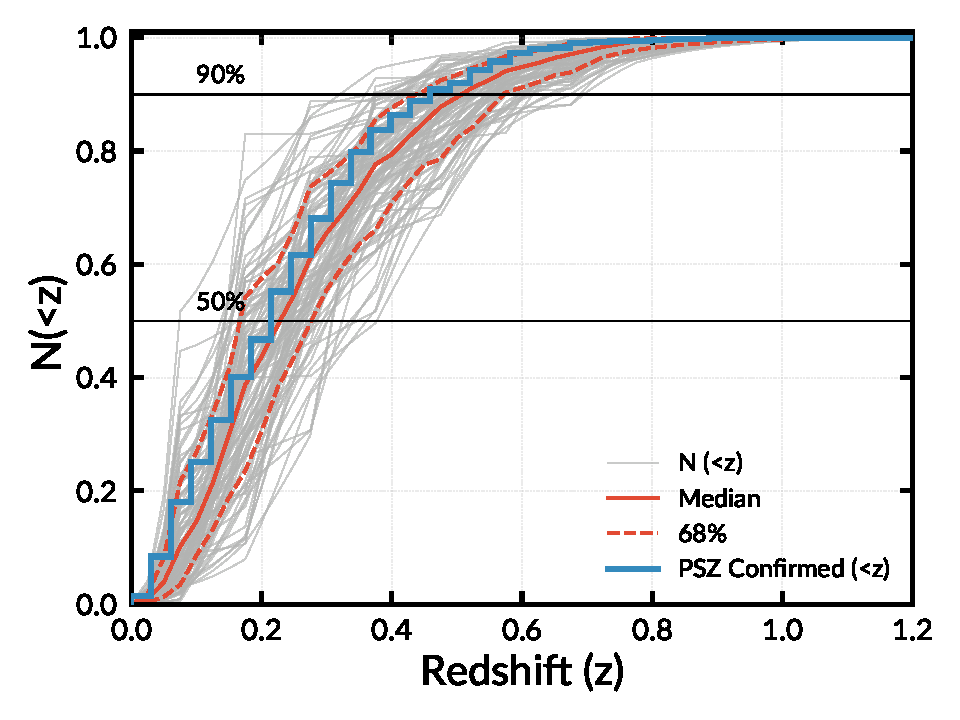
\includegraphics[width=\columnwidth]{figures/cluster_forecast.pdf}
	\caption{Top: The predicted number of clusters as a function of redshift and normalized to unity from the mass function of \cite{Tinker2008}. At each redshift the lower mass limit is given by the mass in the bottom panel at the corresponding redshift. The blue PSZ Confirmed curve shows the normalized, cumulative number of confirmed clusters as a function of redshift. For reference we show the 50\% and 90\% fractional completeness levels. Bottom: Cluster mass as a function of redshift. Redshift bins are the same as \cite{PlanckCollaboration2015a} Figure 27. In each panel the solid and dashed orange lines show the median and region enclosing 68\% of the data respectively.}
	\label{fig:cluster_forecast}
\end{figure}

The first possibility is that the vast majority of clusters in our sample lie at low-$z$. The initial design of our survey uses an $10'\times10'$ search window centered on the PSZ position. Low-$z$ clusters could appear as isolated elliptical galaxies and thus would not be classified as clusters. In follow up inspection of the full--sized mosaics, approximately 1 \degsq, reveals no such low-$z$ structures. In addition, we compute the expected fraction of galaxy clusters as a function of redshift from the cluster mass function of \cite{Tinker2008}. The cluster mass sensitivity of \planck\ varies with redshift (see Figure 27, \citealt{PlanckCollaboration2015a}). To capture this variability, we draw random (with replacement) samples from the confirmed PSZ2 clusters. Because each cluster is previously confirmed the PSZ2 catalog provides an M$_{500c}$ estimate of the total mass. The bottom panel of Figure~\ref{fig:cluster_forecast} shows the cluster mass as a function of redshift, where the gray lines are individual samples and the orange solid and dashed curves are the median and 68\% limits respectively.

The top panel of Figure~\ref{fig:cluster_forecast} shows the expected cumulative distribution of galaxy clusters as a function of redshift.

From these numerical simulations we know that a low fraction ($<5\%$) of all clusters detectable by \planck\ are expected to reside at redshifts less than 0.1. Of the 85 fields observed, we expect approximately four clusters to lie at such low redshifts. We recover three low$-z$ clusters during the course of our analysis.

The second possibility is the vast majority of the clusters in our sample lie at redshifts beyond our optical detection limits. The median limiting \sdssi-band magnitude of our survey is $23.2$ mag, corresponding to a limiting redshift of $z=0.75$ for an \mstar\ galaxy (see Figure~\ref{fig:recovery_redshift}). While it is possible that a number of cluster candidates corresponding to real clusters exists above this redshift, it is unlikely that these correspond to a population of the high SNR objects targeted by this survey. Massive clusters, such as those targeted by this survey, are exceedingly rare objects. For example there are only twelve, currently confirmed, clusters at $z>0.72$ in PSZ2, only five of which are above $z=0.8$. Again, Figure~\ref{fig:cluster_forecast} allows us to estimate the number of clusters missed with our observing limits. At $z>0.7$, we expect $\sim18\%$ of clusters with $M_{500c}=3\times10^{14}~\msol$, corresponding to only fifteen clusters of our 85 observed fields. While high-$z$ objects were expectedly missed by this survey, high-$z$ objects along cannot account for the high number of still unconfirmed clusters. We expect further follow up observations with deep infrared imaging will be required to place further limits on these high-$z$ objects.

\begin{figure}
	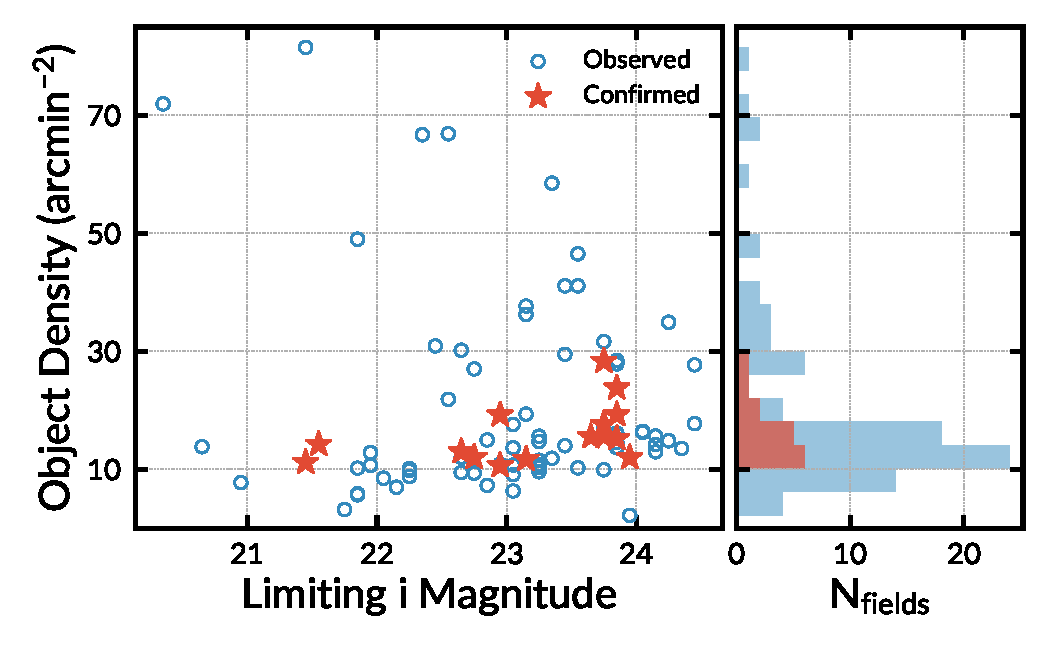
\includegraphics[width=\columnwidth]{figures/N_vs_density.pdf}
	\caption{Right: Object Density in units of number per \arcminsq as a function of the 80\% \sdssi-band limiting magnitude taken from Figure~\ref{fig:recovery_redshift}. Fields where no cluster is identified are given by blue circles and fields with confirmed clusters are shown by orange stars. Left: Histogram of the object surface density of observed fields.}
	\label{fig:N_vs_density}
\end{figure}

The third possibility is that the vast majority of clusters are obscured by the Milky Way. It is possible that the underlying cause for failed cluster identification is confusion from source crowding in our images. If a cluster lies behind a dense foreground of Milky Way sources, then it could be difficult to visually identify the cluster. To estimate the object surface density in our fields, we sum the number of objects reported by \textsc{SExtractor} and dividing by the sky-area of the image. We explore the possibility that we fail to confirm a cluster in the majority of fields because of foreground contamination in Figure~\ref{fig:N_vs_density}. The right panel shows the surface density of objects in the search area as a function of the limiting \sdssi-band magnitude (see also the left panel of Figure~\ref{fig:recovery_redshift}). The right panel shows the number of observed fields with the corresponding object density. In both panels, the fields where we do not identify a cluster is shown in blue, and the successfully identified clusters are in orange.

Our identified clusters fall in a relatively narrow range of object densities, $10-30$ objects \perarcminsq. Roughly two thirds of our fields fall within this range. Of the 31 objects outside our identification range, 15 fields have higher densities. If all fifteen fields contain an obscured cluster we could still not account for the vast majority of fields where we did not identify a cluster, 51 fields or $\sim60\%$ of our observed sample.

Perhaps more interesting are the sixteen fields where the object surface density is lower than our identification range. These are fields where it should be relatively easy to identify a massive cluster should it exist. Of course, the presence of a massive cluster could raise the object density above the lower identification threshold. These fields, especially the fields with deep optical limiting magnitudes are prime candidates for the potential high-$z$ clusters lurking beyond our reach.

The fourth possibility, and perhaps most plausible, is that the vast majority of cluster candidates in our sample are not true $5\sigma$ detections.	In other words, no optical counterpart to the PSZ detection exists. Previous works \citeeg{Barrena2018} find a similar fraction of non-detections, and consider both high noise values in the \planck\ $Y_{500}$ maps \citep{PlanckCollaboration2014a} along with contamination from foreground radio sources. As part of our NED search, we find that approximately 75\% of confirmed PSZ sources have a NVSS radio source (39.6 mJy average flux) within $5'$ of the PSZ position. unconfirmed PSZ sources show slightly fewer sources with approximately 55\% having a NVSS radio source (25.1 mJy average flux) within $5'$.

\section{Summary}\label{sec:summary}

In this work, we report on our analysis of imaging targeting galaxy cluster candidates selected from the second \planck\ all-sky galaxy cluster catalog (PSZ2) \citep{PlanckCollaboration2015a}. We observe 85 candidates with SZ effect SNR $>5$ over the course of seventeen nights spread over three years (2014--2017). We utilize and independently develop a pipeline to process the \sdssg\sdssr\sdssi\sdssz\ imaging taken with both the MOSAIC 1.1 and MOSAIC 3 imagers on the KPNO Mayall-4m telescope (see Section~\ref{sec:data reduction}). We present the first results from the complete data set of 85 fields, eighteen rich galaxy clusters of which fifteen were previously unknown.

After computing accurate photometric redshifts (see Section~\ref{sec:analysis}) we visually inspect each galaxy cluster candidate and adopt stringent confirmation criteria based on the richness, and seperation from the reported PSZ2 position.

The newly discovered clusters range in photometric redshift between $0.13 < z < 0.74$. The upper redshift limit is due to the depth of imaging restricting our ability to reliably detect \lstar\ galaxies to $z<0.9$. Ultimately, this prevents us from finding the most interesting rich clusters at very high redshifts, and will be addressed in a future follow up work.

A large motivation for this work has come from the recent successes of other SZ follow up programs \citeeg{Bayliss2016, Sifon2015a, Kirk2015}. We present this sample of clusters to aid in the confirmation of the PSZ sources, and to potentially reveal clusters with interesting astrophysical properties. The PSZ sources which remain unconfirmed have the potential to be the most interesting.

In future work, we will present the properties of lower richness clusters and small groups of galaxies in addition to multi-wavelength studies using the clusters detected as part of this survey.

\section*{Acknowledgements}
This work was supported by NASA Astrophysics Data Analysis grant number NNX14AF73G and NSF Astronomy and Astrophysics Research Program award number 1615657. We thank the several undergraduate students who worked on this project: August Miller, Alexis Freiling, Jessica Kerman, Kevin Feigelis, Ingrid Zimmerman, and Cole Bisaccia. Alexis, Jessica, and Ingrid were participants in Project SUPER (Science for Undergraduates: A Program for Excellence in Research), a STEM-focused enrichment program through Douglass that offers undergraduate women the opportunity to actively participate in academic research. August participated in the 2014 Rutgers NSF REU program.
This research made use of several open source packages: \textsc{APLpy}, an open-source plotting package for Python hosted at \url{http://aplpy.github.com}; the \textsc{IPython} package \citep{Perez2007}; \textsc{matplotlib}, a Python library for publication quality graphics \citep{Hunter2007} and \textsc{Astropy}, a community developed core Python package for Astronomy \citep{TheAstropyCollaboration2013}.
Funding for the SDSS and SDSS-II has been provided by the Alfred P. Sloan Foundation, the Participating Institutions, the National Science Foundation, the U.S. Department of Energy, the National Aeronautics and Space Administration, the Japanese Monbukagakusho, the Max Planck Society, and the Higher Education Funding Council for England. The SDSS Web Site is \url{http://www.sdss.org/}. The SDSS is managed by the Astrophysical Research Consortium for the Participating Institutions.
This work has made use of data from the European Space Agency (ESA) mission \textit{Gaia} (\url{https://www.cosmos.esa.int/gaia}), processed by the \textit{Gaia} Data Processing and Analysis Consortium (DPAC, \url{https://www.cosmos.esa.int/web/gaia/dpac/consortium}). Funding for the DPAC has been provided by national institutions, in particular the institutions participating in the \textit{Gaia} Multilateral Agreement.
This research has made use of the VizieR catalogue access tool, CDS, Strasbourg, France. The original description of the VizieR service was published in \cite{Ochsenbein2000}.
This research has made use of the SVO Filter Profile Service (\url{http://svo2.cab.inta-csic.es/theory/fps/}) supported from the Spanish MINECO through grant AyA2014-55216.
This research has made use of the NASA/IPAC Extragalactic Database (NED) which is operated by the Jet Propulsion Laboratory, California Institute of Technology, under contract with the National Aeronautics and Space Administration.

%%%%%%%%%%%%%%%%%%%% REFERENCES %%%%%%%%%%%%%%%%%%
% The best way to enter references is to use BibTeX:
\bibliographystyle{apj}
\begin{thebibliography}{}
\expandafter\ifx\csname natexlab\endcsname\relax\def\natexlab#1{#1}\fi

\bibitem[{Abell(1958)}]{Abell1958}
Abell, G.~O. 1958, The Astrophysical Journal Supplement Series, 3, 211

\bibitem[{Aihara {et~al.}(2018)Aihara, Arimoto, Armstrong, Arnouts, Bahcall,
  Bickerton, Bosch, Bundy, Capak, Chan, Chiba, Coupon, Egami, Enoki, Finet,
  Fujimori, Fujimoto, Furusawa, Furusawa, Goto, Goulding, Greco, Greene, Gunn,
  Hamana, Harikane, Hashimoto, Hattori, Hayashi, Hayashi, He{\l}miniak,
  Higuchi, Hikage, Ho, Hsieh, Huang, Huang, Ikeda, Imanishi, Inoue, Iwasawa,
  Iwata, Jaelani, Jian, Kamata, Karoji, Kashikawa, Katayama, Kawanomoto, Kayo,
  Koda, Koike, Kojima, Komiyama, Konno, Koshida, Koyama, Kusakabe, Leauthaud,
  Lee, Lin, Lin, Lupton, Mandelbaum, Matsuoka, Medezinski, Mineo, Miyama,
  Miyatake, Miyazaki, Momose, More, More, Moritani, Moriya, Morokuma, Mukae,
  Murata, Murayama, Nagao, Nakata, Niida, Niikura, Nishizawa, Obuchi, Oguri,
  Oishi, Okabe, Okamoto, Okura, Ono, Onodera, Onoue, Osato, Ouchi, Price, Pyo,
  Sako, Sawicki, Shibuya, Shimasaku, Shimono, Shirasaki, Silverman, Simet,
  Speagle, Spergel, Strauss, Sugahara, Sugiyama, Suto, Suyu, Suzuki, Tait,
  Takada, Takata, Tamura, Tanaka, Tanaka, Tanaka, Tanaka, Terai, Terashima,
  Toba, Tominaga, Toshikawa, Turner, Uchida, Uchiyama, Umetsu, Uraguchi, Urata,
  Usuda, Utsumi, Wang, Wang, Wong, Yabe, Yamada, Yamanoi, Yasuda, Yeh,
  Yonehara, \& Yuma}]{Aihara2018a}
Aihara, H., Arimoto, N., Armstrong, R., {et~al.} 2018, Publications of the
  Astronomical Society of Japan, 70, arXiv:1704.05858

\bibitem[{Albareti {et~al.}(2017)Albareti, Prieto, Almeida, Anders, Anderson,
  Andrews, Arag{\'{o}}n-Salamanca, Argudo-Fern{\'{a}}ndez, Armengaud, Aubourg,
  Avila-Reese, Badenes, Bailey, Barbuy, Barger, Barrera-Ballesteros, Bartosz,
  Basu, Bates, Battaglia, Baumgarten, Baur, Bautista, Beers, Belfiore,
  Bershady, de~Lis, Bird, Bizyaev, Blanc, Blanton, Blomqvist, Bolton,
  Borissova, Bovy, Brandt, Brinkmann, Brownstein, Bundy, Burtin, Busca, Chavez,
  D{\'{i}}az, Cappellari, Carrera, Chen, Cherinka, Cheung, Chiappini,
  Chojnowski, Chuang, Chung, Cirolini, Clerc, Cohen, Comerford, Comparat,
  {Correa do Nascimento}, Cousinou, Covey, Crane, Croft, Cunha, Darling,
  Davidson, Dawson, {Da Costa}, {Da Silva Ilha}, Machado, Delubac, {De Lee},
  {De la Macorra}, {De la Torre}, Diamond-Stanic, Donor, Downes, Drory, Du, {Du
  Mas des Bourboux}, Dwelly, Ebelke, Eigenbrot, Eisenstein, Elsworth, Emsellem,
  Eracleous, Escoffier, Evans, Falc{\'{o}}n-Barroso, Fan, Favole,
  Fernandez-Alvar, Fernandez-Trincado, Feuillet, Fleming, Font-Ribera,
  Freischlad, Frinchaboy, Fu, Gao, Garcia, Garcia-Dias, Garcia-Hern{\'{a}}ndez,
  P{\'{e}}rez, Gaulme, Ge, Geisler, Gillespie, Marin, Girardi, Goddard, Chew,
  Gonzalez-Perez, Grabowski, Green, Grier, Grier, Guo, Guy, Hagen, Hall,
  Harding, Harley, Hasselquist, Hawley, Hayes, Hearty, Hekker, Toledo, Ho,
  Hogg, Holley-Bockelmann, Holtzman, Holzer, Hu, Huber, Hutchinson, Hwang,
  Ibarra-Medel, Ivans, Ivory, Jaehnig, Jensen, Johnson, Jones, Jullo,
  Kallinger, Kinemuchi, Kirkby, Klaene, Kneib, Kollmeier, Lacerna, Lane, Lang,
  Laurent, Law, Leauthaud, {Le Goff}, Li, Li, Li, Li, Liang, Liang, Lima, Lin,
  Lin, Lin, Liu, Long, Lucatello, MacDonald, MacLeod, Mackereth, Mahadevan,
  Maia, Maiolino, Majewski, Malanushenko, Malanushenko, Mallmann, Manchado,
  Maraston, Marques-Chaves, Valpuesta, Masters, Mathur, McGreer, Merloni,
  Merrifield, Mesz{\'{a}}ros, Meza, Miglio, Minchev, Molaverdikhani,
  Montero-Dorta, Mosser, Muna, Myers, Nair, Nandra, Ness, Newman, Nichol,
  Nidever, Nitschelm, O'Connell, Oravetz, Oravetz, Pace, Padilla,
  Palanque-Delabrouille, Pan, Parejko, Paris, Park, Peacock, Peirani,
  Pellejero-Ibanez, Penny, Percival, Percival, Perez-Fournon, Petitjean, Pieri,
  Pinsonneault, Pisani, Prada, Prakash, Price-Jones, Raddick, Rahman, Raichoor,
  Rembold, Reyna, Rich, Richstein, Ridl, Riffel, Riffel, Rix, Robin, Rockosi,
  Rodr{\'{i}}guez-Torres, Rodrigues, Roe, Lopes,
  Rom{\'{a}}n-Z{\'{u}}{\~{n}}iga, Ross, Rossi, Ruan, Ruggeri, Runnoe,
  Salazar-Albornoz, Salvato, Sanchez, Sanchez, Sanchez-Gallego, Santiago,
  Schiavon, Schimoia, Schlafly, Schlegel, Schneider, Sch{\"{o}}nrich,
  Schultheis, Schwope, Seo, Serenelli, Sesar, Shao, Shetrone, Shull, Aguirre,
  Skrutskie, Slosar, Smith, Smith, Sobeck, Somers, Souto, Stark, Stassun,
  Steinmetz, Stello, Bergmann, Strauss, Streblyanska, Stringfellow, Suarez,
  Sun, Taghizadeh-Popp, Tang, Tao, Tayar, Tembe, Thomas, Tinker, Tojeiro,
  Tremonti, Troup, Trump, Unda-Sanzana, Valenzuela, {Van den Bosch},
  Vargas-Maga{\~{n}}a, Vazquez, Villanova, Vivek, Vogt, Wake, Walterbos, Wang,
  Wang, Weaver, Weijmans, Weinberg, Westfall, Whelan, Wilcots, Wild, Williams,
  Wilson, Wood-Vasey, Wylezalek, Xiao, Yan, Yang, Ybarra, Yeche, Yuan,
  Zakamska, Zamora, Zasowski, Zhang, Zhao, Zhao, Zheng, Zheng, Zhou, Zhu, Zinn,
  \& Zou}]{Albareti2017}
Albareti, F.~D., Prieto, C.~A., Almeida, A., {et~al.} 2017, The Astrophysical
  Journal Supplement Series, 233, 25

\bibitem[{Amodeo {et~al.}(2018)Amodeo, Mei, Stanford, Lawrence, Bartlett,
  Stern, Chary, Shim, Marleau, Melin, \&
  Rodr{\'{i}}guez-Gonz{\'{a}}lvez}]{Amodeo2018}
Amodeo, S., Mei, S., Stanford, S.~A., {et~al.} 2018, The Astrophysical Journal,
  853, 36

\bibitem[{Barrena {et~al.}(2018)Barrena, Streblyanska, Ferragamo,
  Rubi{\~{n}}o-Mart{\'{i}}n, Aguado-Barahona, Tramonte, G{\'{e}}nova-Santos,
  Hempel, Lietzen, Aghanim, Arnaud, B{\"{o}}hringer, Chon, Democles, Dahle,
  Douspis, Lasenby, Mazzotta, Melin, Pointecouteau, Pratt, Rossetti, \& van~der
  Burg}]{Barrena2018}
Barrena, R., Streblyanska, A., Ferragamo, A., {et~al.} 2018, Astronomy {\&}
  Astrophysics, 616, A42

\bibitem[{Bauer {et~al.}(2000)Bauer, Condon, Thuan, \& Broderick}]{Bauer2000}
Bauer, F.~E., Condon, J.~J., Thuan, T.~X., \& Broderick, J.~J. 2000, The
  Astrophysical Journal Supplement Series, 129, 547

\bibitem[{Bayliss {et~al.}(2016)Bayliss, Ruel, Stubbs, Allen, Applegate, Ashby,
  Bautz, Benson, Bleem, Bocquet, Brodwin, Capasso, Carlstrom, Chang, Chiu, Cho,
  Clocchiatti, Crawford, Crites, de~Haan, Desai, Dietrich, Dobbs, Doucouliagos,
  Foley, Forman, Garmire, George, Gladders, Gonzalez, Gupta, Halverson,
  Hlavacek-Larrondo, Hoekstra, Holder, Holzapfel, Hou, Hrubes, Huang, Jones,
  Keisler, Knox, Lee, Leitch, von~der Linden, Luong-Van, Mantz, Marrone,
  McDonald, McMahon, Meyer, Mocanu, Mohr, Murray, Padin, Pryke, Rapetti,
  Reichardt, Rest, Ruhl, Saliwanchik, Saro, Sayre, Schaffer, Schrabback,
  Shirokoff, Song, Spieler, Stalder, Stanford, Staniszewski, Stark, Story,
  Vanderlinde, Vieira, Vikhlinin, Williamson, \& Zenteno}]{Bayliss2016}
Bayliss, M.~B., Ruel, J., Stubbs, C.~W., {et~al.} 2016, The Astrophysical
  Journal Supplement Series, 227, 3

\bibitem[{Becker {et~al.}(1995)Becker, White, \& Helfand}]{Becker1995}
Becker, R.~H., White, R.~L., \& Helfand, D.~J. 1995, The Astrophysical Journal,
  450, 559

\bibitem[{Benitez(2000)}]{Benitez2000}
Benitez, N. 2000, The Astrophysical Journal, 536, 571

\bibitem[{Bertin(2006)}]{Bertin2006}
Bertin, E. 2006, in Astronomical Society of the Pacific Conference Series, Vol.
  351, Astronomical Data Analysis Software and Systems XV, ed. C.~Gabriel,
  C.~Arviset, D.~Ponz, \& S.~Enrique, 112

\bibitem[{Bertin \& Arnouts(1996)}]{Bertin1996}
Bertin, E., \& Arnouts, S. 1996, Astronomy and Astrophysics Supplement Series,
  117, 393

\bibitem[{Bertin \& Emmanuel(2011)}]{Bertin2011}
Bertin, E., \& Emmanuel. 2011, Astrophysics Source Code Library, record
  ascl:1110.006

\bibitem[{Bertin {et~al.}(2002)Bertin, Mellier, Radovich, Missonnier, Didelon,
  \& Morin}]{Bertin2002}
Bertin, E., Mellier, Y., Radovich, M., {et~al.} 2002, in Astronomical Society
  of the Pacific Conference Series, Vol. 281, Astronomical Data Analysis
  Software and Systems XI, ed. D.~Bohlender, D.~Durand, \& T.~Handley, 228

\bibitem[{Blanton {et~al.}(2003)Blanton, Hogg, Bahcall, Brinkmann, Britton,
  Connolly, Csabai, Fukugita, Loveday, Meiksin, Munn, Nichol, Okamura, Quinn,
  Schneider, Shimasaku, Strauss, Tegmark, Vogeley, \& Weinberg}]{Blanton2003}
Blanton, M.~R., Hogg, D.~W., Bahcall, N.~A., {et~al.} 2003, The Astrophysical
  Journal, 592, 819

\bibitem[{Bohringer {et~al.}(2000)Bohringer, Voges, Huchra, McLean, Giacconi,
  Rosati, Burg, Mader, Schuecker, Simic, Komossa, Reiprich, Retzlaff, \&
  Trumper}]{Bohringer2000}
Bohringer, H., Voges, W., Huchra, J.~P., {et~al.} 2000, The Astrophysical
  Journal Supplement Series, 129, 435

\bibitem[{Brodwin {et~al.}(2010)Brodwin, Ruel, Ade, Aird, Andersson, Ashby,
  Bautz, Bazin, Benson, Bleem, Carlstrom, Chang, Crawford, Crites, de~Haan,
  Desai, Dobbs, Dudley, Fazio, Foley, Forman, Garmire, George, Gladders,
  Gonzalez, Halverson, High, Holder, Holzapfel, Hrubes, Jones, Joy, Keisler,
  Knox, Lee, Leitch, Lueker, Marrone, McMahon, Mehl, Meyer, Mohr, Montroy,
  Murray, Padin, Plagge, Pryke, Reichardt, Rest, Ruhl, Schaffer, Shaw,
  Shirokoff, Song, Spieler, Stalder, Stanford, Staniszewski, Stark, Stubbs,
  Vanderlinde, Vieira, Vikhlinin, Williamson, Yang, Zahn, \&
  Zenteno}]{Brodwin2010}
Brodwin, M., Ruel, J., Ade, P. A.~R., {et~al.} 2010, The Astrophysical Journal,
  721, 90

\bibitem[{Brown {et~al.}(2016)Brown, Vallenari, Prusti, de~Bruijne, Mignard,
  Drimmel, Babusiaux, Bailer-Jones, Bastian, Biermann, Evans, Eyer, Jansen,
  Jordi, Katz, Klioner, Lammers, Lindegren, Luri, O'Mullane, Panem, Pourbaix,
  Randich, Sartoretti, Siddiqui, Soubiran, Valette, van Leeuwen, Walton, Aerts,
  Arenou, Cropper, H{\o}g, Lattanzi, Grebel, Holland, Huc, Passot, Perryman,
  Bramante, Cacciari, Casta{\~{n}}eda, Chaoul, Cheek, {De Angeli}, Fabricius,
  Guerra, Hern{\'{a}}ndez, Jean-Antoine-Piccolo, Masana, Messineo, Mowlavi,
  Nienartowicz, Ord{\'{o}}{\~{n}}ez-Blanco, Panuzzo, Portell, Richards, Riello,
  Seabroke, Tanga, Th{\'{e}}venin, Torra, Els, Gracia-Abril, Comoretto,
  Garcia-Reinaldos, Lock, Mercier, Altmann, Andrae, Astraatmadja,
  Bellas-Velidis, Benson, Berthier, Blomme, Busso, Carry, Cellino, Clementini,
  Cowell, Creevey, Cuypers, Davidson, {De Ridder}, de~Torres, Delchambre,
  Dell'Oro, Ducourant, Fr{\'{e}}mat, Garc{\'{i}}a-Torres, Gosset, Halbwachs,
  Hambly, Harrison, Hauser, Hestroffer, Hodgkin, Huckle, Hutton, Jasniewicz,
  Jordan, Kontizas, Korn, Lanzafame, Manteiga, Moitinho, Muinonen, Osinde,
  Pancino, Pauwels, Petit, Recio-Blanco, Robin, Sarro, Siopis, Smith, Smith,
  Sozzetti, Thuillot, van Reeven, Viala, Abbas, {Abreu Aramburu}, Accart,
  Aguado, Allan, Allasia, Altavilla, {\'{A}}lvarez, Alves, Anderson, Andrei,
  {Anglada Varela}, Antiche, Antoja, Ant{\'{o}}n, Arcay, Bach, Baker,
  Balaguer-N{\'{u}}{\~{n}}ez, Barache, Barata, Barbier, Barblan, {Barrado y
  Navascu{\'{e}}s}, Barros, Barstow, Becciani, Bellazzini, {Bello
  Garc{\'{i}}a}, Belokurov, Bendjoya, Berihuete, Bianchi, Bienaym{\'{e}},
  Billebaud, Blagorodnova, Blanco-Cuaresma, Boch, Bombrun, Borrachero,
  Bouquillon, Bourda, Bouy, Bragaglia, Breddels, Brouillet, Br{\"{u}}semeister,
  Bucciarelli, Burgess, Burgon, Burlacu, Busonero, Buzzi, Caffau, Cambras,
  Campbell, Cancelliere, Cantat-Gaudin, Carlucci, Carrasco, Castellani,
  Charlot, Charnas, Chiavassa, Clotet, Cocozza, Collins, Costigan, Crifo,
  Cross, Crosta, Crowley, Dafonte, Damerdji, Dapergolas, David, David, {De
  Cat}, de~Felice, de~Laverny, {De Luise}, {De March}, de~Martino, de~Souza,
  Debosscher, del Pozo, Delbo, Delgado, Delgado, {Di Matteo}, Diakite,
  Distefano, Dolding, {Dos Anjos}, Drazinos, Duran, Dzigan, Edvardsson, Enke,
  Evans, {Eynard Bontemps}, Fabre, Fabrizio, Faigler, Falc{\~{a}}o,
  {Farr{\`{a}}s Casas}, Federici, Fedorets, Fern{\'{a}}ndez-Hern{\'{a}}ndez,
  Fernique, Fienga, Figueras, Filippi, Findeisen, Fonti, Fouesneau, Fraile,
  Fraser, Fuchs, Gai, Galleti, Galluccio, Garabato, Garc{\'{i}}a-Sedano,
  Garofalo, Garralda, Gavras, Gerssen, Geyer, Gilmore, Girona, Giuffrida,
  Gomes, Gonz{\'{a}}lez-Marcos, Gonz{\'{a}}lez-N{\'{u}}{\~{n}}ez,
  Gonz{\'{a}}lez-Vidal, Granvik, Guerrier, Guillout, Guiraud, G{\'{u}}rpide,
  Guti{\'{e}}rrez-S{\'{a}}nchez, Guy, Haigron, Hatzidimitriou, Haywood, Heiter,
  Helmi, Hobbs, Hofmann, Holl, Holland, Hunt, Hypki, Icardi, Irwin, {Jevardat
  de Fombelle}, Jofr{\'{e}}, Jonker, Jorissen, Julbe, Karampelas, Kochoska,
  Kohley, Kolenberg, Kontizas, Koposov, Kordopatis, Koubsky, Krone-Martins,
  Kudryashova, Kull, Bachchan, Lacoste-Seris, Lanza, Lavigne, {Le
  Poncin-Lafitte}, Lebreton, Lebzelter, Leccia, Leclerc, Lecoeur-Taibi,
  Lemaitre, Lenhardt, Leroux, Liao, Licata, Lindstr{\o}m, Lister, Livanou,
  Lobel, L{\"{o}}ffler, L{\'{o}}pez, Lorenz, MacDonald, {Magalh{\~{a}}es
  Fernandes}, Managau, Mann, Mantelet, Marchal, Marchant, Marconi, Marinoni,
  Marrese, Marschalk{\'{o}}, Marshall, Mart{\'{i}}n-Fleitas, Martino, Mary,
  Matijevi{\v{c}}, Mazeh, McMillan, Messina, Michalik, Millar, Miranda, Molina,
  Molinaro, Molinaro, Moln{\'{a}}r, Moniez, Montegriffo, Mor, Mora, Morbidelli,
  Morel, Morgenthaler, Morris, Mulone, Muraveva, Musella, Narbonne, Nelemans,
  Nicastro, Noval, Ord{\'{e}}novic, Ordieres-Mer{\'{e}}, Osborne, Pagani,
  Pagano, Pailler, Palacin, Palaversa, Parsons, Pecoraro, Pedrosa,
  Pentik{\"{a}}inen, Pichon, Piersimoni, Pineau, Plachy, Plum, Poujoulet,
  Pr{\v{s}}a, Pulone, Ragaini, Rago, Rambaux, Ramos-Lerate, Ranalli, Rauw,
  Read, Regibo, Reyl{\'{e}}, Ribeiro, Rimoldini, Ripepi, Riva, Rixon, Roelens,
  Romero-G{\'{o}}mez, Rowell, Royer, Ruiz-Dern, Sadowski, {Sagrist{\`{a}}
  Sell{\'{e}}s}, Sahlmann, Salgado, Salguero, Sarasso, Savietto, Schultheis,
  Sciacca, Segol, Segovia, Segransan, Shih, Smareglia, Smart, Solano, Solitro,
  Sordo, {Soria Nieto}, Souchay, Spagna, Spoto, Stampa, Steele,
  Steidelm{\"{u}}ller, Stephenson, Stoev, Suess, S{\"{u}}veges, Surdej,
  Szabados, Szegedi-Elek, Tapiador, Taris, Tauran, Taylor, Teixeira, Terrett,
  Tingley, Trager, Turon, Ulla, Utrilla, Valentini, van Elteren, {Van
  Hemelryck}, van Leeuwen, Varadi, Vecchiato, Veljanoski, Via, Vicente, Vogt,
  Voss, Votruba, Voutsinas, Walmsley, Weiler, Weingrill, Wevers, Wyrzykowski,
  Yoldas, {\v{Z}}erjal, Zucker, Zurbach, Zwitter, Alecu, Allen, {Allende
  Prieto}, Amorim, Anglada-Escud{\'{e}}, Arsenijevic, Azaz, Balm, Beck,
  Bernstein, Bigot, Bijaoui, Blasco, Bonfigli, Bono, Boudreault, Bressan,
  Brown, Brunet, Bunclark, Buonanno, Butkevich, Carret, Carrion, Chemin,
  Ch{\'{e}}reau, Corcione, Darmigny, de~Boer, de~Teodoro, de~Zeeuw, {Delle
  Luche}, Domingues, Dubath, Fodor, Fr{\'{e}}zouls, Fries, Fustes, Fyfe,
  Gallardo, Gallegos, Gardiol, Gebran, Gomboc, G{\'{o}}mez, Grux, Gueguen,
  Heyrovsky, Hoar, Iannicola, {Isasi Parache}, Janotto, Joliet, Jonckheere,
  Keil, Kim, Klagyivik, Klar, Knude, Kochukhov, Kolka, Kos, Kutka, Lainey,
  LeBouquin, Liu, Loreggia, Makarov, Marseille, Martayan, Martinez-Rubi,
  Massart, Meynadier, Mignot, Munari, Nguyen, Nordlander, Ocvirk, O'Flaherty,
  {Olias Sanz}, Ortiz, Osorio, Oszkiewicz, Ouzounis, Palmer, Park, Pasquato,
  Peltzer, Peralta, P{\'{e}}turaud, Pieniluoma, Pigozzi, Poels, Prat,
  Prod'homme, Raison, Rebordao, Risquez, Rocca-Volmerange, Rosen, Ruiz-Fuertes,
  Russo, Sembay, {Serraller Vizcaino}, Short, Siebert, Silva, Sinachopoulos,
  Slezak, Soffel, Sosnowska, Strai{\v{z}}ys, ter Linden, Terrell, Theil, Tiede,
  Troisi, Tsalmantza, Tur, Vaccari, Vachier, Valles, {Van Hamme}, Veltz,
  Virtanen, Wallut, Wichmann, Wilkinson, Ziaeepour, \&
  Zschocke}]{GaiaCollaboration2016}
Brown, A. G.~A., Vallenari, A., Prusti, T., {et~al.} 2016, Astronomy {\&}
  Astrophysics, 595, A2

\bibitem[{Bruzual \& Charlot(2003)}]{Bruzual2003}
Bruzual, G., \& Charlot, S. 2003, Monthly Notices of the Royal Astronomical
  Society, 344, 1000

\bibitem[{Burenin(2017)}]{Burenin2017}
Burenin, R.~A. 2017, Astronomy Letters, 43, 507

\bibitem[{Carlstrom {et~al.}(2011)Carlstrom, Ade, Aird, Benson, Bleem, Busetti,
  Chang, Chauvin, Cho, Crawford, Crites, Dobbs, Halverson, Heimsath, Holzapfel,
  Hrubes, Joy, Keisler, Lanting, Lee, Leitch, Leong, Lu, Lueker, Luong-Van,
  McMahon, Mehl, Meyer, Mohr, Montroy, Padin, Plagge, Pryke, Ruhl, Schaffer,
  Schwan, Shirokoff, Spieler, Staniszewski, Stark, Tucker, Vanderlinde, Vieira,
  \& Williamson}]{Carlstrom2011}
Carlstrom, J.~E., Ade, P. A.~R., Aird, K.~A., {et~al.} 2011, Publications of
  the Astronomical Society of the Pacific, 123, 568

\bibitem[{Chabrier(2003)}]{Chabrier2003}
Chabrier, G. 2003, Publications of the Astronomical Society of the Pacific,
  115, 763

\bibitem[{Chambers {et~al.}(2016)Chambers, Magnier, Metcalfe, Flewelling,
  Huber, Waters, Denneau, Draper, Farrow, Finkbeiner, Holmberg, Koppenhoefer,
  Price, Saglia, Schlafly, Smartt, Sweeney, Wainscoat, Burgett, Grav, Heasley,
  Hodapp, Jedicke, Kaiser, Kudritzki, Luppino, Lupton, Monet, Morgan, Onaka,
  Stubbs, Tonry, Banados, Bell, Bender, Bernard, Botticella, Casertano,
  Chastel, Chen, Chen, Cole, Deacon, Frenk, Fitzsimmons, Gezari, Goessl,
  Goggia, Goldman, Grebel, Hambly, Hasinger, Heavens, Heckman, Henderson,
  Henning, Holman, Hopp, Ip, Isani, Keyes, Koekemoer, Kotak, Long, Lucey, Liu,
  Martin, McLean, Morganson, Murphy, Nieto-Santisteban, Norberg, Peacock, Pier,
  Postman, Primak, Rae, Rest, Riess, Riffeser, Rix, Roser, Schilbach, Schultz,
  Scolnic, Szalay, Seitz, Shiao, Small, Smith, Soderblom, Taylor, Thakar,
  Thiel, Thilker, Urata, Valenti, Walter, Watters, Werner, White, Wood-Vasey,
  \& Wyse}]{Chambers2016}
Chambers, K.~C., Magnier, E.~A., Metcalfe, N., {et~al.} 2016, eprint
  arXiv:1612.05560, arXiv:1612.05560

\bibitem[{Coe {et~al.}(2006)Coe, Benitez, Sanchez, Jee, Bouwens, \&
  Ford}]{Coe2006}
Coe, D., Benitez, N., Sanchez, S.~F., {et~al.} 2006, The Astronomical Journal,
  132, 926

\bibitem[{Condon {et~al.}(1998)Condon, Cotton, Greisen, Yin, Perley, Taylor, \&
  Broderick}]{Condon1998}
Condon, J.~J., Cotton, W.~D., Greisen, E.~W., {et~al.} 1998, The Astronomical
  Journal, 115, 1693

\bibitem[{Dahle {et~al.}(2003)Dahle, Pedersen, Lilje, Maddox, \&
  Kaiser}]{Dahle2003}
Dahle, H., Pedersen, K., Lilje, P.~B., Maddox, S.~J., \& Kaiser, N. 2003, The
  Astrophysical Journal, 591, 662

\bibitem[{Dahlen {et~al.}(2013)Dahlen, Mobasher, Faber, Ferguson, Barro,
  Finkelstein, Finlator, Fontana, Gruetzbauch, Johnson, Pforr, Salvato,
  Wiklind, Wuyts, Acquaviva, Dickinson, Guo, Huang, Huang, Newman, Bell,
  Conselice, Galametz, Gawiser, Giavalisco, Grogin, Hathi, Kocevski, Koekemoer,
  Koo, Lee, McGrath, Papovich, Peth, Ryan, Somerville, Weiner, \&
  Wilson}]{Dahlen2013}
Dahlen, T., Mobasher, B., Faber, S.~M., {et~al.} 2013, The Astrophysical
  Journal, 775, 93

\bibitem[{{Dark Energy Survey Collaboration} {et~al.}(2016){Dark Energy Survey
  Collaboration}, Abbott, Abdalla, Allam, Aleksic, Amara, Bacon, Balbinot,
  Banerji, Bechtol, Benoit-Levy, Bernstein, Bertin, Blazek, Dodelson, Bonnett,
  Brooks, Bridle, Brunner, Buckley-Geer, Burke, Capozzi, Caminha, Carlsen,
  Carnero-Rosell, Carollo, Carrasco-Kind, Carretero, Castander, Clerkin,
  Collett, Conselice, Crocce, Cunha, D'Andrea, da~Costa, Davis, Desai, Diehl,
  Dietrich, Doel, Drlica-Wagner, Etherington, Estrada, Evrard, Fabbri, Finley,
  Flaugher, Fosalba, Foley, Frieman, Garcia-Bellido, Gaztanaga, Gerdes,
  Giannantonio, Goldstein, Gruen, Gruendl, Guarnieri, Gutierrez, Hartley,
  Honscheid, Jain, James, Jeltema, Jouvel, Kessler, King, Kirk, Kron, Kuehn,
  Kuropatkin, Lahav, Li, Lima, Lin, Maia, Makler, Manera, Maraston, Marshall,
  Martini, McMahon, Melchior, Merson, Miller, Miquel, Mohr, Morice-Atkinson,
  Naidoo, Neilsen, Nichol, Nord, Ogando, Ostrovski, Palmese, Papadopoulos,
  Peiris, Peoples, Plazas, Percival, Reed, Romer, Roodman, Ross, Rozo, Rykoff,
  Sadeh, Sako, Sanchez, Sanchez, Santiago, Scarpine, Schubnell, Sevilla-Noarbe,
  Sheldon, Smith, Smith, Soares-Santos, Sobreira, Soumagnac, Suchyta, Sullivan,
  Swanson, Tarle, Thaler, Thomas, Thomas, Tucker, Vieira, Vikram, Walker,
  Wechsler, Wester, Weller, Whiteway, Wilcox, Yanny, Zhang, Zuntz, \&
  Zuntz}]{DarkEnergySurveyCollaboration2016}
{Dark Energy Survey Collaboration}, D. E.~S., Abbott, T., Abdalla, F.~B.,
  {et~al.} 2016, Monthly Notices of the Royal Astronomical Society, 460, 1270

\bibitem[{de~Vaucouleurs(1948)}]{DeVaucouleurs1948}
de~Vaucouleurs, G. 1948, Annales d'Astrophysique, 11, 247

\bibitem[{Douglas {et~al.}(1996)Douglas, Bash, Bozyan, Torrence, \&
  Wolfe}]{Douglas1996}
Douglas, J.~N., Bash, F.~N., Bozyan, F.~A., Torrence, G.~W., \& Wolfe, C. 1996,
  The Astronomical Journal, 111, 1945

\bibitem[{Flewelling {et~al.}(2016)Flewelling, Magnier, Chambers, Heasley,
  Holmberg, Huber, Sweeney, Waters, Chen, Farrow, Hasinger, Henderson, Long,
  Metcalfe, Nieto-Santisteban, Norberg, Saglia, Szalay, Rest, Thakar, Tonry,
  Valenti, Werner, White, Denneau, Draper, Hodapp, Jedicke, Kaiser, Kudritzki,
  Price, Wainscoat, Chastel, McClean, Postman, \& Shiao}]{Flewelling2016}
Flewelling, H.~A., Magnier, E.~A., Chambers, K.~C., {et~al.} 2016, eprint
  arXiv:1612.05243, arXiv:1612.05243

\bibitem[{Foley {et~al.}(2011)Foley, Andersson, Bazin, de~Haan, Ruel, Ade,
  Aird, Armstrong, Ashby, Bautz, Benson, Bleem, Bonamente, Brodwin, Carlstrom,
  Chang, Clocchiatti, Crawford, Crites, Desai, Dobbs, Dudley, Fazio, Forman,
  Garmire, George, Gladders, Gonzalez, Halverson, High, Holder, Holzapfel,
  Hoover, Hrubes, Jones, Joy, Keisler, Knox, Lee, Leitch, Lueker, Luong-Van,
  Marrone, McMahon, Mehl, Meyer, Mohr, Montroy, Murray, Padin, Plagge, Pryke,
  Reichardt, Rest, Ruhl, Saliwanchik, Saro, Schaffer, Shaw, Shirokoff, Song,
  Spieler, Stalder, Stanford, Staniszewski, Stark, Story, Stubbs, Vanderlinde,
  Vieira, Vikhlinin, Williamson, \& Zenteno}]{Foley2011}
Foley, R.~J., Andersson, K., Bazin, G., {et~al.} 2011, The Astrophysical
  Journal, 731, 86

\bibitem[{Harris {et~al.}(1990)Harris, Forman, Gioia, Hale, Harnden, Jones,
  Karakashian, Maccacaro, McSweeney, \& Primini}]{Harris1990}
Harris, D.~E., Forman, W., Gioia, I.~M., {et~al.} 1990, The Einstein
  Observatory catalog of IPC X ray sources. Volume 4E: Right ascension range
  08h 00m to 11h 59m, by D.E. Harris et al. Smithsonian Astrophysical
  Observatory, 1990, 4

\bibitem[{Harrison \& Coles(2012)}]{Harrison2012}
Harrison, I., \& Coles, P. 2012, Monthly Notices of the Royal Astronomical
  Society: Letters, 421, L19

\bibitem[{Harrison \& Hotchkiss(2013)}]{Harrison2013}
Harrison, I., \& Hotchkiss, S. 2013, Journal of Cosmology and Astroparticle
  Physics, 2013, 022

\bibitem[{Hasselfield {et~al.}(2013)Hasselfield, Hilton, Marriage, Addison,
  Barrientos, Battaglia, Battistelli, Bond, Crichton, Das, Devlin, Dicker,
  Dunkley, D{\"{u}}nner, Fowler, Gralla, Hajian, Halpern, Hincks, Hlozek,
  Hughes, Infante, Irwin, Kosowsky, Marsden, Menanteau, Moodley, Niemack,
  Nolta, Page, Partridge, Reese, Schmitt, Sehgal, Sherwin, Sievers,
  Sif{\'{o}}n, Spergel, Staggs, Swetz, Switzer, Thornton, Trac, \&
  Wollack}]{Hasselfield2013a}
Hasselfield, M., Hilton, M., Marriage, T.~A., {et~al.} 2013, Journal of
  Cosmology and Astroparticle Physics, 2013, 008

\bibitem[{H{\o}g {et~al.}(2000)H{\o}g, Fabricius, Makarov, Urban, Corbin,
  Wycoff, Bastian, Schwekendiek, \& Wicenec}]{Hog2000}
H{\o}g, E., Fabricius, C., Makarov, V.~V., {et~al.} 2000, Astronomy and
  Astrophysics, 355, L27

\bibitem[{Hogg {et~al.}(2002)Hogg, Baldry, Blanton, \& Eisenstein}]{Hogg2002}
Hogg, D.~W., Baldry, I.~K., Blanton, M.~R., \& Eisenstein, D.~J. 2002, eprint
  arXiv:astro-ph/0210394, arXiv:0210394

\bibitem[{Huchra {et~al.}(1990)Huchra, Geller, Henry, \& Postman}]{Huchra1990}
Huchra, J.~P., Geller, M.~J., Henry, J.~P., \& Postman, M. 1990, The
  Astrophysical Journal, 365, 66

\bibitem[{Hunter(2007)}]{Hunter2007}
Hunter, J.~D. 2007, Computing in Science {\&} Engineering, 9, 90

\bibitem[{Ilbert {et~al.}(2009)Ilbert, Capak, Salvato, Aussel, McCracken,
  Sanders, Scoville, Kartaltepe, Arnouts, Floc'h, Mobasher, Taniguchi,
  Lamareille, Leauthaud, Sasaki, Thompson, Zamojski, Zamorani, Bardelli,
  Bolzonella, Bongiorno, Brusa, Caputi, Carollo, Contini, Cook, Coppa,
  Cucciati, de~la Torre, de~Ravel, Franzetti, Garilli, Hasinger, Iovino,
  Kampczyk, Kneib, Knobel, Kovac, {Le Borgne}, {Le Brun}, F?vre, Lilly, Looper,
  Maier, Mainieri, Mellier, Mignoli, Murayama, Pell?, Peng, P?rez-Montero,
  Renzini, Ricciardelli, Schiminovich, Scodeggio, Shioya, Silverman, Surace,
  Tanaka, Tasca, Tresse, Vergani, \& Zucca}]{Ilbert2009}
Ilbert, O., Capak, P., Salvato, M., {et~al.} 2009, The Astrophysical Journal,
  690, 1236

\bibitem[{Jenkins {et~al.}(2001)Jenkins, Frenk, White, Colberg, Cole, Evrard,
  Couchman, \& Yoshida}]{Jenkins2001}
Jenkins, A., Frenk, C.~S., White, S. D.~M., {et~al.} 2001, Monthly Notices of
  the Royal Astronomical Society, 321, 372

\bibitem[{Kirk {et~al.}(2015)Kirk, Hilton, Cress, Crawford, Hughes, Battaglia,
  Bond, Burke, Gralla, Hajian, Hasselfield, Hincks, Infante, Kosowsky,
  Marriage, Menanteau, Moodley, Niemack, Sievers, Sifon, Wilson, Wollack, \&
  Zunckel}]{Kirk2015}
Kirk, B., Hilton, M., Cress, C., {et~al.} 2015, Monthly Notices of the Royal
  Astronomical Society, 449, 4010

\bibitem[{Komatsu {et~al.}(2011)Komatsu, Smith, Dunkley, Bennett, Gold,
  Hinshaw, Jarosik, Larson, Nolta, Page, Spergel, Halpern, Hill, Kogut, Limon,
  Meyer, Odegard, Tucker, Weiland, Wollack, \& Wright}]{Komatsu2011}
Komatsu, E., Smith, K.~M., Dunkley, J., {et~al.} 2011, The Astrophysical
  Journal Supplement Series, 192, 18

\bibitem[{Liu {et~al.}(2015)Liu, Hennig, Desai, Hoyle, Koppenhoefer, Mohr,
  Paech, Burgett, Chambers, Cole, Draper, Kaiser, Metcalfe, Morgan, Price,
  Stubbs, Tonry, Wainscoat, \& Waters}]{Liu2015a}
Liu, J., Hennig, C., Desai, S., {et~al.} 2015, Monthly Notices of the Royal
  Astronomical Society, 449, 3370

\bibitem[{{LSST Dark Energy Science Collaboration}(2012)}]{LSST2012}
{LSST Dark Energy Science Collaboration}. 2012, arXiv preprint arXiv:1211.0310,
  133

\bibitem[{Menanteau {et~al.}(2009)Menanteau, Hughes, Jimenez,
  Hernandez-Monteagudo, Verde, Kosowsky, Moodley, Infante, \&
  Roche}]{Menanteau2009a}
Menanteau, F., Hughes, J.~P., Jimenez, R., {et~al.} 2009, The Astrophysical
  Journal, 698, 1221

\bibitem[{Menanteau {et~al.}(2010{\natexlab{a}})Menanteau, Hughes, Barrientos,
  Deshpande, Hilton, Infante, Jimenez, Kosowsky, Moodley, Spergel, \&
  Verde}]{Menanteau2010}
Menanteau, F., Hughes, J.~P., Barrientos, L.~F., {et~al.} 2010{\natexlab{a}},
  The Astrophysical Journal Supplement Series, 191, 340

\bibitem[{Menanteau {et~al.}(2010{\natexlab{b}})Menanteau, Gonz{\'{a}}lez,
  Juin, Marriage, Reese, Acquaviva, Aguirre, Appel, Baker, Barrientos,
  Battistelli, Bond, Das, Deshpande, Devlin, Dicker, Dunkley, D{\"{u}}nner,
  Essinger-Hileman, Fowler, Hajian, Halpern, Hasselfield,
  Hern{\'{a}}ndez-Monteagudo, Hilton, Hincks, Hlozek, Huffenberger, Hughes,
  Infante, Irwin, Klein, Kosowsky, Lin, Marsden, Moodley, Niemack, Nolta, Page,
  Parker, Partridge, Sehgal, Sievers, Spergel, Staggs, Swetz, Switzer,
  Thornton, Trac, Warne, \& Wollack}]{Menanteau2010a}
Menanteau, F., Gonz{\'{a}}lez, J., Juin, J.-B., {et~al.} 2010{\natexlab{b}},
  The Astrophysical Journal, 723, 1523

\bibitem[{Menanteau {et~al.}(2012)Menanteau, Hughes, Sif{\'{o}}n, Hilton,
  Gonz?lez, Infante, {Felipe Barrientos}, Baker, Bond, Das, Devlin, Dunkley,
  Hajian, Hincks, Kosowsky, Marsden, Marriage, Moodley, Niemack, Nolta, Page,
  Reese, Sehgal, Sievers, Spergel, Staggs, \& Wollack}]{Menanteau2012}
Menanteau, F., Hughes, J.~P., Sif{\'{o}}n, C., {et~al.} 2012, The Astrophysical
  Journal, 748, 7

\bibitem[{Menanteau {et~al.}(2013)Menanteau, Sif{\'{o}}n, Barrientos,
  Battaglia, Bond, Crichton, Das, Devlin, Dicker, D{\"{u}}nner, Gralla, Hajian,
  Hasselfield, Hilton, Hincks, Hughes, Infante, Kosowsky, Marriage, Marsden,
  Moodley, Niemack, Nolta, Page, Partridge, Reese, Schmitt, Sievers, Spergel,
  Staggs, Switzer, \& Wollack}]{Menanteau2013}
Menanteau, F., Sif{\'{o}}n, C., Barrientos, L.~F., {et~al.} 2013, The
  Astrophysical Journal, 765, 67

\bibitem[{Michel \& Huchra(1988)}]{Michel1988}
Michel, A., \& Huchra, J. 1988, Publications of the Astronomical Society of the
  Pacific, 100, 1423

\bibitem[{Molino {et~al.}(2017)Molino, Ben{\'{i}}tez, Ascaso, Coe, Postman,
  Jouvel, Host, Lahav, Seitz, Medezinski, Rosati, Schoenell, Koekemoer,
  Jimenez-Teja, Broadhurst, Melchior, Balestra, Bartelmann, Bouwens, Bradley,
  Czakon, Donahue, Ford, Graur, Graves, Grillo, Infante, Jha, Kelson, Lazkoz,
  Lemze, Maoz, Mercurio, Meneghetti, Merten, Moustakas, Nonino, Orgaz, Riess,
  Rodney, Sayers, Umetsu, Zheng, \& Zitrin}]{Molino2017}
Molino, A., Ben{\'{i}}tez, N., Ascaso, B., {et~al.} 2017, Monthly Notices of
  the Royal Astronomical Society, 470, 95

\bibitem[{Mommert(2017)}]{Mommert2017}
Mommert, M. 2017, Astronomy and Computing, 18, 47

\bibitem[{Mortonson {et~al.}(2010)Mortonson, Hu, \& Huterer}]{Mortonson2011}
Mortonson, M.~J., Hu, W., \& Huterer, D. 2010, Physical Review D, 83, 023015

\bibitem[{Ochsenbein {et~al.}(2000)Ochsenbein, Bauer, \&
  Marcout}]{Ochsenbein2000}
Ochsenbein, F., Bauer, P., \& Marcout, J. 2000, Astronomy and Astrophysics
  Supplement Series, 143, 23

\bibitem[{Oke(1974)}]{Oke1974}
Oke, J.~B. 1974, The Astrophysical Journal Supplement Series, 27, 21

\bibitem[{Perez \& Granger(2007)}]{Perez2007}
Perez, F., \& Granger, B.~E. 2007, Computing in Science {\&} Engineering, 9, 21

\bibitem[{{Planck Collaboration} {et~al.}(2011){Planck Collaboration}, Ade,
  Aghanim, Arnaud, Ashdown, Aumont, Baccigalupi, Baker, Balbi, Banday,
  Barreiro, Bartlett, Battaner, Benabed, Bennett, Beno{\^{i}}t, Bernard,
  Bersanelli, Bhatia, Bock, Bonaldi, Bond, Borrill, Bouchet, Bradshaw, Bremer,
  Bucher, Burigana, Butler, Cabella, Cantalupo, Cappellini, Cardoso, Carr,
  Casale, Catalano, Cay{\'{o}}n, Challinor, Chamballu, Charra, Chary, Chiang,
  Chiang, Christensen, Clements, Colombi, Couchot, Coulais, Crill, Crone,
  Crook, Cuttaia, Danese, D'Arcangelo, Davies, Davis, de~Bernardis, de~Bruin,
  de~Gasperis, de~Rosa, de~Zotti, Delabrouille, Delouis, D{\'{e}}sert, Dick,
  Dickinson, Dolag, Dole, Donzelli, Dor{\'{e}}, D{\"{o}}rl, Douspis, Dupac,
  Efstathiou, En{\ss}lin, Eriksen, Finelli, Foley, Forni, Fosalba, Frailis,
  Franceschi, Freschi, Gaier, Galeotta, Gallegos, Gandolfo, Ganga, Giard,
  Giardino, Gienger, Giraud-H{\'{e}}raud, Gonz{\'{a}}lez, Gonz{\'{a}}lez-Nuevo,
  G{\'{o}}rski, Gratton, Gregorio, Gruppuso, Guyot, Haissinski, Hansen,
  Harrison, Helou, Henrot-Versill{\'{e}}, Hern{\'{a}}ndez-Monteagudo, Herranz,
  Hildebrandt, Hivon, Hobson, Holmes, Hornstrup, Hovest, Hoyland, Huffenberger,
  Jaffe, Jagemann, Jones, Juillet, Juvela, Kangaslahti, Keih{\"{a}}nen,
  Keskitalo, Kisner, Kneissl, Knox, Krassenburg, Kurki-Suonio, Lagache,
  L{\"{a}}hteenm{\"{a}}ki, Lamarre, Lange, Lasenby, Laureijs, Lawrence, Leach,
  Leahy, Leonardi, Leroy, Lilje, Linden-V{\o}rnle, L{\'{o}}pez-Caniego, Lowe,
  Lubin, Mac{\'{i}}as-P{\'{e}}rez, Maciaszek, MacTavish, Maffei, Maino,
  Mandolesi, Mann, Maris, Mart{\'{i}}nez-Gonz{\'{a}}lez, Masi, Massardi,
  Matarrese, Matthai, Mazzotta, McDonald, McGehee, Meinhold, Melchiorri, Melin,
  Mendes, Mennella, Mevi, Miniscalco, Mitra, Miville-Desch{\^{e}}nes, Moneti,
  Montier, Morgante, Morisset, Mortlock, Munshi, Murphy, Naselsky, Natoli,
  Netterfield, N{\o}rgaard-Nielsen, Noviello, Novikov, Novikov, O'Dwyer, Ortiz,
  Osborne, Osuna, Oxborrow, Pajot, Paladini, Partridge, Pasian, Passvogel,
  Patanchon, Pearson, Pearson, Perdereau, Perotto, Perrotta, Piacentini, Piat,
  Pierpaoli, Plaszczynski, Platania, Pointecouteau, Polenta, Ponthieu, Popa,
  Poutanen, Pr{\'{e}}zeau, Prunet, Puget, Rachen, Reach, Rebolo, Reinecke,
  Reix, Renault, Ricciardi, Riller, Ristorcelli, Rocha, Rosset, Rowan-Robinson,
  Rubi{\~{n}}o-Mart{\'{i}}n, Rusholme, Salerno, Sandri, Santos, Savini,
  Schaefer, Scott, Seiffert, Shellard, Simonetto, Smoot, Sozzi, Starck,
  Sternberg, Stivoli, Stolyarov, Stompor, Stringhetti, Sudiwala, Sunyaev,
  Sygnet, Tapiador, Tauber, Tavagnacco, Taylor, Terenzi, Texier, Toffolatti,
  Tomasi, Torre, Tristram, Tuovinen, T{\"{u}}rler, Tuttlebee, Umana,
  Valenziano, Valiviita, Varis, Vibert, Vielva, Villa, Vittorio, Wade, Wandelt,
  Watson, White, White, Wilkinson, Yvon, Zacchei, Zonca, \&
  Zonca}]{PlanckCollaboration2011}
{Planck Collaboration}, Ade, P. A.~R., Aghanim, N., {et~al.} 2011, Astronomy
  {\&} Astrophysics, 536, A1

\bibitem[{{Planck Collaboration} {et~al.}(2014{\natexlab{a}}){Planck
  Collaboration}, Ade, Aghanim, Armitage-Caplan, Arnaud, Ashdown,
  Atrio-Barandela, Aumont, Baccigalupi, Banday, Barreiro, Barrena, Bartlett,
  Battaner, Battye, Benabed, Beno{\^{i}}t, Benoit-L{\'{e}}vy, Bernard,
  Bersanelli, Bielewicz, Bikmaev, Blanchard, Bobin, Bock, B{\"{o}}hringer,
  Bonaldi, Bond, Borrill, Bouchet, Bourdin, Bridges, Brown, Bucher, Burenin,
  Burigana, Butler, Cardoso, Carvalho, Catalano, Challinor, Chamballu, Chary,
  Chiang, Chiang, Chon, Christensen, Church, Clements, Colombi, Colombo,
  Couchot, Coulais, Crill, Curto, Cuttaia, {Da Silva}, Dahle, Danese, Davies,
  Davis, de~Bernardis, de~Rosa, de~Zotti, Delabrouille, Delouis,
  D{\'{e}}mocl{\`{e}}s, D{\'{e}}sert, Dickinson, Diego, Dolag, Dole, Donzelli,
  Dor{\'{e}}, Douspis, Dupac, Efstathiou, En{\ss}lin, Eriksen, Finelli,
  Flores-Cacho, Forni, Frailis, Franceschi, Fromenteau, Galeotta, Ganga,
  G{\'{e}}nova-Santos, Giard, Giardino, Giraud-H{\'{e}}raud,
  Gonz{\'{a}}lez-Nuevo, G{\'{o}}rski, Gratton, Gregorio, Gruppuso, Hansen,
  Hanson, Harrison, Henrot-Versill{\'{e}}, Hern{\'{a}}ndez-Monteagudo, Herranz,
  Hildebrandt, Hivon, Hobson, Holmes, Hornstrup, Hovest, Huffenberger, Hurier,
  Jaffe, Jaffe, Jones, Juvela, Keih{\"{a}}nen, Keskitalo, Khamitov, Kisner,
  Kneissl, Knoche, Knox, Kunz, Kurki-Suonio, Lagache, L{\"{a}}hteenm{\"{a}}ki,
  Lamarre, Lasenby, Laureijs, Lawrence, Leahy, Leonardi, Le{\'{o}}n-Tavares,
  Lesgourgues, Liddle, Liguori, Lilje, Linden-V{\o}rnle, L{\'{o}}pez-Caniego,
  Lubin, Mac{\'{i}}as-P{\'{e}}rez, Maffei, Maino, Mandolesi, Marcos-Caballero,
  Maris, Marshall, Martin, Mart{\'{i}}nez-Gonz{\'{a}}lez, Masi, Matarrese,
  Matthai, Mazzotta, Meinhold, Melchiorri, Melin, Mendes, Mennella, Migliaccio,
  Mitra, Miville-Desch{\^{e}}nes, Moneti, Montier, Morgante, Mortlock, Moss,
  Munshi, Naselsky, Nati, Natoli, Netterfield, N{\o}rgaard-Nielsen, Noviello,
  Novikov, Novikov, Osborne, Oxborrow, Paci, Pagano, Pajot, Paoletti,
  Partridge, Pasian, Patanchon, Perdereau, Perotto, Perrotta, Piacentini, Piat,
  Pierpaoli, Pietrobon, Plaszczynski, Pointecouteau, Polenta, Ponthieu, Popa,
  Poutanen, Pratt, Pr{\'{e}}zeau, Prunet, Puget, Rachen, Rebolo, Reinecke,
  Remazeilles, Renault, Ricciardi, Riller, Ristorcelli, Rocha, Roman, Rosset,
  Roudier, Rowan-Robinson, Rubi{\~{n}}o-Mart{\'{i}}n, Rusholme, Sandri, Santos,
  Savini, Scott, Seiffert, Shellard, Spencer, Starck, Stolyarov, Stompor,
  Sudiwala, Sunyaev, Sureau, Sutton, Suur-Uski, Sygnet, Tauber, Tavagnacco,
  Terenzi, Toffolatti, Tomasi, Tristram, Tucci, Tuovinen, T{\"{u}}rler, Umana,
  Valenziano, Valiviita, {Van Tent}, Vielva, Villa, Vittorio, Wade, Wandelt,
  Weller, White, White, Yvon, Zacchei, \& Zonca}]{PlanckCollaboration2014a}
---. 2014{\natexlab{a}}, Astronomy {\&} Astrophysics, 571, A20

\bibitem[{{Planck Collaboration} {et~al.}(2014{\natexlab{b}}){Planck
  Collaboration}, Ade, Aghanim, Armitage-Caplan, Arnaud, Ashdown,
  Atrio-Barandela, Aumont, Aussel, Baccigalupi, Banday, Barreiro, Barrena,
  Bartelmann, Bartlett, Battaner, Benabed, Beno{\^{i}}t, Benoit-L{\'{e}}vy,
  Bernard, Bersanelli, Bielewicz, Bikmaev, Bobin, Bock, B{\"{o}}hringer,
  Bonaldi, Bond, Borrill, Bouchet, Bridges, Bucher, Burenin, Burigana, Butler,
  Cardoso, Carvalho, Catalano, Challinor, Chamballu, Chary, Chen, Chiang,
  Chiang, Chon, Christensen, Churazov, Church, Clements, Colombi, Colombo,
  Comis, Couchot, Coulais, Crill, Curto, Cuttaia, {Da Silva}, Dahle, Danese,
  Davies, Davis, de~Bernardis, de~Rosa, de~Zotti, Delabrouille, Delouis,
  D{\'{e}}mocl{\`{e}}s, D{\'{e}}sert, Dickinson, Diego, Dolag, Dole, Donzelli,
  Dor{\'{e}}, Douspis, Dupac, Efstathiou, Eisenhardt, En{\ss}lin, Eriksen,
  Feroz, Finelli, Flores-Cacho, Forni, Frailis, Franceschi, Fromenteau,
  Galeotta, Ganga, G{\'{e}}nova-Santos, Giard, Giardino, Gilfanov,
  Giraud-H{\'{e}}raud, Gonz{\'{a}}lez-Nuevo, G{\'{o}}rski, Grainge, Gratton,
  Gregorio, {Groeneboom, N}, Gruppuso, Hansen, Hanson, Harrison, Hempel,
  Henrot-Versill{\'{e}}, Hern{\'{a}}ndez-Monteagudo, Herranz, Hildebrandt,
  Hivon, Hobson, Holmes, Hornstrup, Hovest, Huffenberger, Hurier,
  Hurley-Walker, Jaffe, Jaffe, Jones, Juvela, Keih{\"{a}}nen, Keskitalo,
  Khamitov, Kisner, Kneissl, Knoche, Knox, Kunz, Kurki-Suonio, Lagache,
  L{\"{a}}hteenm{\"{a}}ki, Lamarre, Lasenby, Laureijs, Lawrence, Leahy,
  Leonardi, Le{\'{o}}n-Tavares, Lesgourgues, Li, Liddle, Liguori, Lilje,
  Linden-V{\o}rnle, L{\'{o}}pez-Caniego, Lubin, Mac{\'{i}}as-P{\'{e}}rez,
  MacTavish, Maffei, Maino, Mandolesi, Maris, Marshall, Martin,
  Mart{\'{i}}nez-Gonz{\'{a}}lez, Masi, Massardi, Matarrese, Matthai, Mazzotta,
  Mei, Meinhold, Melchiorri, Melin, Mendes, Mennella, Migliaccio, Mikkelsen,
  Mitra, Miville-Desch{\^{e}}nes, Moneti, Montier, Morgante, Mortlock, Munshi,
  Murphy, Naselsky, Nati, Natoli, Nesvadba, Netterfield, N{\o}rgaard-Nielsen,
  Noviello, Novikov, Novikov, O'Dwyer, Olamaie, Osborne, Oxborrow, Paci,
  Pagano, Pajot, Paoletti, Pasian, Patanchon, Pearson, Perdereau, Perotto,
  Perrott, Perrotta, Piacentini, Piat, Pierpaoli, Pietrobon, Plaszczynski,
  Pointecouteau, Polenta, Ponthieu, Popa, Poutanen, Pratt, Pr{\'{e}}zeau,
  Prunet, Puget, Rachen, Reach, Rebolo, Reinecke, Remazeilles, Renault,
  Ricciardi, Riller, Ristorcelli, Rocha, Rosset, Roudier, Rowan-Robinson,
  Rubi{\~{n}}o-Mart{\'{i}}n, Rumsey, Rusholme, Sandri, Santos, Saunders,
  Savini, Schammel, Scott, Seiffert, Shellard, Shimwell, Spencer, Stanford,
  Starck, Stolyarov, Stompor, Sudiwala, Sunyaev, Sureau, Sutton, Suur-Uski,
  Sygnet, Tauber, Tavagnacco, Terenzi, Toffolatti, Tomasi, Tristram, Tucci,
  Tuovinen, T{\"{u}}rler, Umana, Valenziano, Valiviita, {Van Tent}, Vibert,
  Vielva, Villa, Vittorio, Wade, Wandelt, White, White, Yvon, Zacchei, \&
  Zonca}]{PlanckCollaboration2014}
---. 2014{\natexlab{b}}, Astronomy {\&} Astrophysics, 571, A29

\bibitem[{{Planck Collaboration} {et~al.}(2015{\natexlab{a}}){Planck
  Collaboration}, Ade, Aghanim, Arnaud, Ashdown, Aumont, Baccigalupi, Banday,
  Barreiro, Barrena, Bartlett, Bartolo, Battaner, Battye, Benabed,
  Beno{\^{i}}t, Benoit-L{\'{e}}vy, Bernard, Bersanelli, Bielewicz, Bikmaev,
  B{\"{o}}hringer, Bonaldi, Bonavera, Bond, Borrill, Bouchet, Bucher, Burenin,
  Burigana, Butler, Calabrese, Cardoso, Carvalho, Catalano, Challinor,
  Chamballu, Chary, Chiang, Chon, Christensen, Clements, Colombi, Colombo,
  Combet, Comis, Couchot, Coulais, Crill, Curto, Cuttaia, Dahle, Danese,
  Davies, Davis, de~Bernardis, de~Rosa, de~Zotti, Delabrouille, D{\'{e}}sert,
  Dickinson, Diego, Dolag, Dole, Donzelli, Dor{\'{e}}, Douspis, Ducout, Dupac,
  Efstathiou, Eisenhardt, Elsner, En{\ss}lin, Eriksen, Falgarone, Fergusson,
  Feroz, Ferragamo, Finelli, Forni, Frailis, Fraisse, Franceschi, Frejsel,
  Galeotta, Galli, Ganga, G{\'{e}}nova-Santos, Giard, Giraud-H{\'{e}}raud,
  Gjerl{\o}w, Gonz{\'{a}}lez-Nuevo, G{\'{o}}rski, Grainge, Gratton, Gregorio,
  Gruppuso, Gudmundsson, Hansen, Hanson, Harrison, Hempel,
  Henrot-Versill{\'{e}}, Hern{\'{a}}ndez-Monteagudo, Herranz, Hildebrandt,
  Hivon, Hobson, Holmes, Hornstrup, Hovest, Huffenberger, Hurier, Jaffe, Jaffe,
  Jin, Jones, Juvela, Keih{\"{a}}nen, Keskitalo, Khamitov, Kisner, Kneissl,
  Knoche, Kunz, Kurki-Suonio, Lagache, Lamarre, Lasenby, Lattanzi, Lawrence,
  Leonardi, Lesgourgues, Levrier, Liguori, Lilje, Linden-V{\o}rnle,
  L{\'{o}}pez-Caniego, Lubin, Mac{\'{i}}as-P{\'{e}}rez, Maggio, Maino, Mak,
  Mandolesi, Mangilli, Martin, Mart{\'{i}}nez-Gonz{\'{a}}lez, Masi, Matarrese,
  Mazzotta, McGehee, Mei, Melchiorri, Melin, Mendes, Mennella, Migliaccio,
  Mitra, Miville-Desch{\^{e}}nes, Moneti, Montier, Morgante, Mortlock, Moss,
  Munshi, Murphy, Naselsky, Nastasi, Nati, Natoli, Netterfield,
  N{\o}rgaard-Nielsen, Noviello, Novikov, Novikov, Olamaie, Oxborrow, Paci,
  Pagano, Pajot, Paoletti, Pasian, Patanchon, Pearson, Perdereau, Perotto,
  Perrott, Perrotta, Pettorino, Piacentini, Piat, Pierpaoli, Pietrobon,
  Plaszczynski, Pointecouteau, Polenta, Pratt, Pr{\'{e}}zeau, Prunet, Puget,
  Rachen, Reach, Rebolo, Reinecke, Remazeilles, Renault, Renzi, Ristorcelli,
  Rocha, Rosset, Rossetti, Roudier, Rozo, Rubi{\~{n}}o-Mart{\'{i}}n, Rumsey,
  Rusholme, Rykoff, Sandri, Santos, Saunders, Savelainen, Savini, Schammel,
  Scott, Seiffert, Shellard, Shimwell, Spencer, Stanford, Stern, Stolyarov,
  Stompor, Streblyanska, Sudiwala, Sunyaev, Sutton, Suur-Uski, Sygnet, Tauber,
  Terenzi, Toffolatti, Tomasi, Tramonte, Tristram, Tucci, Tuovinen, Umana,
  Valenziano, Valiviita, {Van Tent}, Vielva, Villa, Wade, Wandelt, Wehus,
  White, Wright, Yvon, Zacchei, \& Zonca}]{PlanckCollaboration2015a}
---. 2015{\natexlab{a}}, Astronomy {\&} Astrophysics, 594, A27

\bibitem[{{Planck Collaboration} {et~al.}(2015{\natexlab{b}}){Planck
  Collaboration}, Ade, Aghanim, Arnaud, Ashdown, Aumont, Baccigalupi, Banday,
  Barreiro, Barrena, Bartolo, Battaner, Benabed, Benoit-L{\'{e}}vy, Bernard,
  Bersanelli, Bielewicz, Bikmaev, B{\"{o}}hringer, Bonaldi, Bonavera, Bond,
  Borrill, Bouchet, Burenin, Burigana, Butler, Calabrese, Carvalho, Catalano,
  Chamballu, Chiang, Chon, Christensen, Churazov, Clements, Colombo, Comis,
  Couchot, Curto, Cuttaia, Dahle, Danese, Davies, Davis, de~Bernardis, de~Rosa,
  de~Zotti, Delabrouille, Diego, Dole, Dor{\'{e}}, Douspis, Ducout, Dupac,
  Efstathiou, Elsner, En{\ss}lin, Eriksen, Finelli, Flores-Cacho, Forni,
  Frailis, Fraisse, Franceschi, Frejsel, Fromenteau, Galeotta, Ganga,
  G{\'{e}}nova-Santos, Giard, Gilfanov, Giraud-H{\'{e}}raud, Gjerl{\o}w,
  Gonz{\'{a}}lez-Nuevo, G{\'{o}}rski, Gruppuso, Hansen, Hanson, Harrison,
  Hempel, Henrot-Versill{\'{e}}, Hern{\'{a}}ndez-Monteagudo, Herranz,
  Hildebrandt, Hivon, Hobson, Holmes, Hornstrup, Hovest, Huffenberger, Hurier,
  Jaffe, Jones, Juvela, Keih{\"{a}}nen, Keskitalo, Khamitov, Kisner, Kneissl,
  Knoche, Kunz, Kurki-Suonio, Lagache, Lamarre, Lasenby, Lattanzi, Lawrence,
  Leonardi, Levrier, Liguori, Lilje, Linden-V{\o}rnle, L{\'{o}}pez-Caniego,
  Lubin, Mac{\'{i}}as-P{\'{e}}rez, Maino, Mandolesi, Maris, Martin,
  Mart{\'{i}}nez-Gonz{\'{a}}lez, Masi, Matarrese, Mazzotta, Melin, Mendes,
  Mennella, Migliaccio, Miville-Desch{\^{e}}nes, Moneti, Montier, Morgante,
  Mortlock, Munshi, Murphy, Naselsky, Nati, Natoli, N{\o}rgaard-Nielsen,
  Novikov, Novikov, Oxborrow, Pagano, Pajot, Paoletti, Pasian, Perdereau,
  Perotto, Perrotta, Pettorino, Piacentini, Piat, Pietrobon, Plaszczynski,
  Pointecouteau, Polenta, Popa, Pratt, Prunet, Puget, Rachen, Reinecke,
  Remazeilles, Renault, Ricciardi, Ristorcelli, Rocha, Roman, Rosset, Rossetti,
  Roudier, Rubi{\~{n}}o-Mart{\'{i}}n, Rusholme, Sandri, Scott, Spencer,
  Stolyarov, Sudiwala, Sunyaev, Sutton, Suur-Uski, Sygnet, Tauber, Terenzi,
  Toffolatti, Tomasi, Tristram, Tucci, Valenziano, Valiviita, {Van Tent},
  Vibert, Vielva, Villa, Wade, Wandelt, Wehus, Yvon, Zacchei, \&
  Zonca}]{PlanckCollaboration2015}
---. 2015{\natexlab{b}}, Astronomy {\&} Astrophysics, 582, A29

\bibitem[{{Planck Collaboration} {et~al.}(2016){Planck Collaboration}, Ade,
  Aghanim, Arnaud, Ashdown, Aumont, Baccigalupi, Banday, Barreiro, Barrena,
  Bartolo, Battaner, Benabed, Benoit-L{\'{e}}vy, Bernard, Bersanelli,
  Bielewicz, Bikmaev, B{\"{o}}hringer, Bonaldi, Bonavera, Bond, Borrill,
  Bouchet, Burenin, Burigana, Calabrese, Cardoso, Catalano, Chamballu, Chary,
  Chiang, Chon, Christensen, Clements, Colombo, Combet, Comis, Crill, Curto,
  Cuttaia, Dahle, Danese, Davies, Davis, de~Bernardis, de~Rosa, de~Zotti,
  Delabrouille, Diego, Dole, Donzelli, Dor{\'{e}}, Douspis, Dupac, Efstathiou,
  Elsner, En{\ss}lin, Eriksen, Ferragamo, Finelli, Forni, Frailis, Fraisse,
  Franceschi, Fromenteau, Galeotta, Galli, Ganga, G{\'{e}}nova-Santos, Giard,
  Gjerl{\o}w, Gonz{\'{a}}lez-Nuevo, G{\'{o}}rski, Gruppuso, Hansen, Harrison,
  Hempel, Hern{\'{a}}ndez-Monteagudo, Herranz, Hildebrandt, Hivon, Hornstrup,
  Hovest, Huffenberger, Hurier, Jaffe, Keih{\"{a}}nen, Keskitalo, Khamitov,
  Kisner, Kneissl, Knoche, Kunz, Kurki-Suonio, Lamarre, Lasenby, Lattanzi,
  Lawrence, Leonardi, Le{\'{o}}n-Tavares, Levrier, Lietzen, Liguori, Lilje,
  Linden-V{\o}rnle, L{\'{o}}pez-Caniego, Lubin, Mac{\'{i}}as-P{\'{e}}rez,
  Maffei, Maino, Mandolesi, Maris, Martin, Mart{\'{i}}nez-Gonz{\'{a}}lez, Masi,
  Matarrese, McGehee, Melchiorri, Mennella, Migliaccio,
  Miville-Desch{\^{e}}nes, Moneti, Montier, Morgante, Mortlock, Munshi, Murphy,
  Naselsky, Nati, Natoli, Novikov, Novikov, Oxborrow, Pagano, Pajot, Paoletti,
  Pasian, Perdereau, Pettorino, Piacentini, Piat, Pierpaoli, Plaszczynski,
  Pointecouteau, Polenta, Pratt, Prunet, Puget, Rachen, Rebolo, Reinecke,
  Remazeilles, Renault, Renzi, Ristorcelli, Rocha, Rosset, Rossetti, Roudier,
  Rubi{\~{n}}o-Mart{\'{i}}n, Rusholme, Sandri, Santos, Savelainen, Savini,
  Scott, Stolyarov, Streblyanska, Sudiwala, Sunyaev, Suur-Uski, Sygnet, Tauber,
  Terenzi, Toffolatti, Tomasi, Tramonte, Tristram, Tucci, Valenziano,
  Valiviita, {Van Tent}, Vielva, Villa, Wade, Wandelt, Wehus, Yvon, Zacchei, \&
  Zonca}]{PlanckCollaboration2016a}
---. 2016, Astronomy {\&} Astrophysics, 586, A139

\bibitem[{Prusti {et~al.}(2016)Prusti, de~Bruijne, Brown, Vallenari, Babusiaux,
  Bailer-Jones, Bastian, Biermann, Evans, Eyer, Jansen, Jordi, Klioner,
  Lammers, Lindegren, Luri, Mignard, Milligan, Panem, Poinsignon, Pourbaix,
  Randich, Sarri, Sartoretti, Siddiqui, Soubiran, Valette, van Leeuwen, Walton,
  Aerts, Arenou, Cropper, Drimmel, H{\o}g, Katz, Lattanzi, O'Mullane, Grebel,
  Holland, Huc, Passot, Bramante, Cacciari, Casta{\~{n}}eda, Chaoul, Cheek, {De
  Angeli}, Fabricius, Guerra, Hern{\'{a}}ndez, Jean-Antoine-Piccolo, Masana,
  Messineo, Mowlavi, Nienartowicz, Ord{\'{o}}{\~{n}}ez-Blanco, Panuzzo,
  Portell, Richards, Riello, Seabroke, Tanga, Th{\'{e}}venin, Torra, Els,
  Gracia-Abril, Comoretto, Garcia-Reinaldos, Lock, Mercier, Altmann, Andrae,
  Astraatmadja, Bellas-Velidis, Benson, Berthier, Blomme, Busso, Carry,
  Cellino, Clementini, Cowell, Creevey, Cuypers, Davidson, {De Ridder},
  de~Torres, Delchambre, Dell'Oro, Ducourant, Fr{\'{e}}mat,
  Garc{\'{i}}a-Torres, Gosset, Halbwachs, Hambly, Harrison, Hauser, Hestroffer,
  Hodgkin, Huckle, Hutton, Jasniewicz, Jordan, Kontizas, Korn, Lanzafame,
  Manteiga, Moitinho, Muinonen, Osinde, Pancino, Pauwels, Petit, Recio-Blanco,
  Robin, Sarro, Siopis, Smith, Smith, Sozzetti, Thuillot, van Reeven, Viala,
  Abbas, {Abreu Aramburu}, Accart, Aguado, Allan, Allasia, Altavilla,
  {\'{A}}lvarez, Alves, Anderson, Andrei, {Anglada Varela}, Antiche, Antoja,
  Ant{\'{o}}n, Arcay, Atzei, Ayache, Bach, Baker, Balaguer-N{\'{u}}{\~{n}}ez,
  Barache, Barata, Barbier, Barblan, Baroni, {Barrado y Navascu{\'{e}}s},
  Barros, Barstow, Becciani, Bellazzini, Bellei, {Bello Garc{\'{i}}a},
  Belokurov, Bendjoya, Berihuete, Bianchi, Bienaym{\'{e}}, Billebaud,
  Blagorodnova, Blanco-Cuaresma, Boch, Bombrun, Borrachero, Bouquillon, Bourda,
  Bouy, Bragaglia, Breddels, Brouillet, Br{\"{u}}semeister, Bucciarelli,
  Budnik, Burgess, Burgon, Burlacu, Busonero, Buzzi, Caffau, Cambras, Campbell,
  Cancelliere, Cantat-Gaudin, Carlucci, Carrasco, Castellani, Charlot, Charnas,
  Charvet, Chassat, Chiavassa, Clotet, Cocozza, Collins, Collins, Costigan,
  Crifo, Cross, Crosta, Crowley, Dafonte, Damerdji, Dapergolas, David, David,
  {De Cat}, de~Felice, de~Laverny, {De Luise}, {De March}, de~Martino,
  de~Souza, Debosscher, del Pozo, Delbo, Delgado, Delgado, di~Marco, {Di
  Matteo}, Diakite, Distefano, Dolding, {Dos Anjos}, Drazinos, Dur{\'{a}}n,
  Dzigan, Ecale, Edvardsson, Enke, Erdmann, Escolar, Espina, Evans, {Eynard
  Bontemps}, Fabre, Fabrizio, Faigler, Falc{\~{a}}o, {Farr{\`{a}}s Casas},
  Faye, Federici, Fedorets, Fern{\'{a}}ndez-Hern{\'{a}}ndez, Fernique, Fienga,
  Figueras, Filippi, Findeisen, Fonti, Fouesneau, Fraile, Fraser, Fuchs,
  Furnell, Gai, Galleti, Galluccio, Garabato, Garc{\'{i}}a-Sedano, Gar{\'{e}},
  Garofalo, Garralda, Gavras, Gerssen, Geyer, Gilmore, Girona, Giuffrida,
  Gomes, Gonz{\'{a}}lez-Marcos, Gonz{\'{a}}lez-N{\'{u}}{\~{n}}ez,
  Gonz{\'{a}}lez-Vidal, Granvik, Guerrier, Guillout, Guiraud, G{\'{u}}rpide,
  Guti{\'{e}}rrez-S{\'{a}}nchez, Guy, Haigron, Hatzidimitriou, Haywood, Heiter,
  Helmi, Hobbs, Hofmann, Holl, Holland, Hunt, Hypki, Icardi, Irwin, {Jevardat
  de Fombelle}, Jofr{\'{e}}, Jonker, Jorissen, Julbe, Karampelas, Kochoska,
  Kohley, Kolenberg, Kontizas, Koposov, Kordopatis, Koubsky, Kowalczyk,
  Krone-Martins, Kudryashova, Kull, Bachchan, Lacoste-Seris, Lanza, Lavigne,
  {Le Poncin-Lafitte}, Lebreton, Lebzelter, Leccia, Leclerc, Lecoeur-Taibi,
  Lemaitre, Lenhardt, Leroux, Liao, Licata, Lindstr{\o}m, Lister, Livanou,
  Lobel, L{\"{o}}ffler, L{\'{o}}pez, Lopez-Lozano, Lorenz, Loureiro, MacDonald,
  {Magalh{\~{a}}es Fernandes}, Managau, Mann, Mantelet, Marchal, Marchant,
  Marconi, Marie, Marinoni, Marrese, Marschalk{\'{o}}, Marshall,
  Mart{\'{i}}n-Fleitas, Martino, Mary, Matijevi{\v{c}}, Mazeh, McMillan,
  Messina, Mestre, Michalik, Millar, Miranda, Molina, Molinaro, Molinaro,
  Moln{\'{a}}r, Moniez, Montegriffo, Monteiro, Mor, Mora, Morbidelli, Morel,
  Morgenthaler, Morley, Morris, Mulone, Muraveva, Musella, Narbonne, Nelemans,
  Nicastro, Noval, Ord{\'{e}}novic, Ordieres-Mer{\'{e}}, Osborne, Pagani,
  Pagano, Pailler, Palacin, Palaversa, Parsons, Paulsen, Pecoraro, Pedrosa,
  Pentik{\"{a}}inen, Pereira, Pichon, Piersimoni, Pineau, Plachy, Plum,
  Poujoulet, Pr{\v{s}}a, Pulone, Ragaini, Rago, Rambaux, Ramos-Lerate, Ranalli,
  Rauw, Read, Regibo, Renk, Reyl{\'{e}}, Ribeiro, Rimoldini, Ripepi, Riva,
  Rixon, Roelens, Romero-G{\'{o}}mez, Rowell, Royer, Rudolph, Ruiz-Dern,
  Sadowski, {Sagrist{\`{a}} Sell{\'{e}}s}, Sahlmann, Salgado, Salguero,
  Sarasso, Savietto, Schnorhk, Schultheis, Sciacca, Segol, Segovia, Segransan,
  Serpell, Shih, Smareglia, Smart, Smith, Solano, Solitro, Sordo, {Soria
  Nieto}, Souchay, Spagna, Spoto, Stampa, Steele, Steidelm{\"{u}}ller,
  Stephenson, Stoev, Suess, S{\"{u}}veges, Surdej, Szabados, Szegedi-Elek,
  Tapiador, Taris, Tauran, Taylor, Teixeira, Terrett, Tingley, Trager, Turon,
  Ulla, Utrilla, Valentini, van Elteren, {Van Hemelryck}, van Leeuwen, Varadi,
  Vecchiato, Veljanoski, Via, Vicente, Vogt, Voss, Votruba, Voutsinas,
  Walmsley, Weiler, Weingrill, Werner, Wevers, Whitehead, Wyrzykowski, Yoldas,
  {\v{Z}}erjal, Zucker, Zurbach, Zwitter, Alecu, Allen, {Allende Prieto},
  Amorim, Anglada-Escud{\'{e}}, Arsenijevic, Azaz, Balm, Beck, Bernstein,
  Bigot, Bijaoui, Blasco, Bonfigli, Bono, Boudreault, Bressan, Brown, Brunet,
  Bunclark, Buonanno, Butkevich, Carret, Carrion, Chemin, Ch{\'{e}}reau,
  Corcione, Darmigny, de~Boer, de~Teodoro, de~Zeeuw, {Delle Luche}, Domingues,
  Dubath, Fodor, Fr{\'{e}}zouls, Fries, Fustes, Fyfe, Gallardo, Gallegos,
  Gardiol, Gebran, Gomboc, G{\'{o}}mez, Grux, Gueguen, Heyrovsky, Hoar,
  Iannicola, {Isasi Parache}, Janotto, Joliet, Jonckheere, Keil, Kim,
  Klagyivik, Klar, Knude, Kochukhov, Kolka, Kos, Kutka, Lainey, LeBouquin, Liu,
  Loreggia, Makarov, Marseille, Martayan, Martinez-Rubi, Massart, Meynadier,
  Mignot, Munari, Nguyen, Nordlander, Ocvirk, O'Flaherty, {Olias Sanz}, Ortiz,
  Osorio, Oszkiewicz, Ouzounis, Palmer, Park, Pasquato, Peltzer, Peralta,
  P{\'{e}}turaud, Pieniluoma, Pigozzi, Poels, Prat, Prod'homme, Raison,
  Rebordao, Risquez, Rocca-Volmerange, Rosen, Ruiz-Fuertes, Russo, Sembay,
  {Serraller Vizcaino}, Short, Siebert, Silva, Sinachopoulos, Slezak, Soffel,
  Sosnowska, Strai{\v{z}}ys, ter Linden, Terrell, Theil, Tiede, Troisi,
  Tsalmantza, Tur, Vaccari, Vachier, Valles, {Van Hamme}, Veltz, Virtanen,
  Wallut, Wichmann, Wilkinson, Ziaeepour, \& Zschocke}]{GaiaCollaboration2016a}
Prusti, T., de~Bruijne, J. H.~J., Brown, A. G.~A., {et~al.} 2016, Astronomy
  {\&} Astrophysics, 595, A1

\bibitem[{Reichardt {et~al.}(2013)Reichardt, Stalder, Bleem, Montroy, Aird,
  Andersson, Armstrong, Ashby, Bautz, Bayliss, Bazin, Benson, Brodwin,
  Carlstrom, Chang, Cho, Clocchiatti, Crawford, Crites, de~Haan, Desai, Dobbs,
  Dudley, Foley, Forman, George, Gladders, Gonzalez, Halverson, Harrington,
  High, Holder, Holzapfel, Hoover, Hrubes, Jones, Joy, Keisler, Knox, Lee,
  Leitch, Liu, Lueker, Luong-Van, Mantz, Marrone, McDonald, McMahon, Mehl,
  Meyer, Mocanu, Mohr, Murray, Natoli, Padin, Plagge, Pryke, Rest, Ruel, Ruhl,
  Saliwanchik, Saro, Sayre, Schaffer, Shaw, Shirokoff, Song, Spieler,
  Staniszewski, Stark, Story, Stubbs, {\v{S}}uhada, van Engelen, Vanderlinde,
  Vieira, Vikhlinin, Williamson, Zahn, \& Zenteno}]{Reichardt2013}
Reichardt, C.~L., Stalder, B., Bleem, L.~E., {et~al.} 2013, The Astrophysical
  Journal, 763, 127

\bibitem[{Sif{\'{o}}n {et~al.}(2016)Sif{\'{o}}n, Battaglia, Hasselfield,
  Menanteau, Barrientos, Bond, Crichton, Devlin, D{\"{u}}nner, Hilton, Hincks,
  Hlozek, Huffenberger, Hughes, Infante, Kosowsky, Marsden, Marriage, Moodley,
  Niemack, Page, Spergel, Staggs, Trac, \& Wollack}]{Sifon2015a}
Sif{\'{o}}n, C., Battaglia, N., Hasselfield, M., {et~al.} 2016, Monthly Notices
  of the Royal Astronomical Society, 461, 248

\bibitem[{Streblyanska {et~al.}(2018)Streblyanska, Barrena, Rubino-Martin,
  van~der Burg, Aghanim, Aguado-Barahona, Ferragamo, \&
  Lietzen}]{Streblyanska2018}
Streblyanska, A., Barrena, R., Rubino-Martin, J.~A., {et~al.} 2018, eprint
  arXiv:1804.01356, arXiv:1804.01356

\bibitem[{Sunyaev \& Zeldovich(1972)}]{Sunyaev1972}
Sunyaev, R.~A., \& Zeldovich, Y.~B. 1972, Comments on Astrophysics and Space
  Physics, 4

\bibitem[{Swetz {et~al.}(2011)Swetz, Ade, Amiri, Appel, Battistelli, Burger,
  Chervenak, Devlin, Dicker, Doriese, D{\"{u}}nner, Essinger-Hileman, Fisher,
  Fowler, Halpern, Hasselfield, Hilton, Hincks, Irwin, Jarosik, Kaul, Klein,
  Lau, Limon, Marriage, Marsden, Martocci, Mauskopf, Moseley, Netterfield,
  Niemack, Nolta, Page, Parker, Staggs, Stryzak, Switzer, Thornton, Tucker,
  Wollack, \& Zhao}]{Swetz2011}
Swetz, D.~S., Ade, P. A.~R., Amiri, M., {et~al.} 2011, The Astrophysical
  Journal Supplement Series, 194, 41

\bibitem[{Tauber {et~al.}(2010)Tauber, Mandolesi, Puget, Banos, Bersanelli,
  Bouchet, Butler, Charra, Crone, Dodsworth, Efstathiou, Gispert, Guyot,
  Gregorio, Juillet, Lamarre, Laureijs, Lawrence, N{\o}rgaard-Nielsen,
  Passvogel, Reix, Texier, Vibert, Zacchei, Ade, Aghanim, Aja, Alippi, Aloy,
  Armand, Arnaud, Arondel, Arreola-Villanueva, Artal, Artina, Arts, Ashdown,
  Aumont, Azzaro, Bacchetta, Baccigalupi, Baker, Balasini, Balbi, Banday,
  Barbier, Barreiro, Bartelmann, Battaglia, Battaner, Benabed, Beney, Beneyton,
  Bennett, Benoit, Bernard, Bhandari, Bhatia, Biggi, Biggins, Billig, Blanc,
  Blavot, Bock, Bonaldi, Bond, Bonis, Borders, Borrill, Boschini, Boulanger,
  Bouvier, Bouzit, Bowman, Br{\'{e}}elle, Bradshaw, Braghin, Bremer, Brienza,
  Broszkiewicz, Burigana, Burkhalter, Cabella, Cafferty, Cairola, Caminade,
  Camus, Cantalupo, Cappellini, Cardoso, Carr, Catalano, Cay{\'{o}}n, Cesa,
  Chaigneau, Challinor, Chamballu, Chambelland, Charra, Chiang, Chlewicki,
  Christensen, Church, Ciancietta, Cibrario, Cizeron, Clements, Collaudin,
  Colley, Colombi, Colombo, Colombo, Corre, Couchot, Cougrand, Coulais, Couzin,
  Crane, Crill, Crook, Crumb, Cuttaia, D{\"{o}}rl, da~Silva, Daddato, Damasio,
  Danese, D'Aquino, D'Arcangelo, Dassas, Davies, Davies, Davis, {De Bernardis},
  de~Chambure, de~Gasperis, {De la Fuente}, {De Paco}, {De Rosa}, {De Troia},
  {De Zotti}, Dehamme, Delabrouille, Delouis, D{\'{e}}sert, di~Girolamo,
  Dickinson, Doelling, Dolag, Domken, Douspis, Doyle, Du, Dubruel, Dufour,
  Dumesnil, Dupac, Duret, Eder, Elfving, En{\ss}lin, Eng, English, Eriksen,
  Estaria, Falvella, Ferrari, Finelli, Fishman, Fogliani, Foley, Fonseca,
  Forma, Forni, Fosalba, Fourmond, Frailis, Franceschet, Franceschi,
  Fran{\c{c}}ois, Frerking, G{\'{o}}mez-Re{\~{n}}asco, G{\'{o}}rski, Gaier,
  Galeotta, Ganga, {Garc{\'{i}}a L{\'{a}}zaro}, Garnica, Gaspard, Gavila,
  Giard, Giardino, Gienger, Giraud-Heraud, Glorian, Griffin, Gruppuso,
  Guglielmi, Guichon, Guillaume, Guillouet, Haissinski, Hansen, Hardy,
  Harrison, Hazell, Hechler, Heckenauer, Heinzer, Hell, Henrot-Versill{\'{e}},
  Hern{\'{a}}ndez-Monteagudo, Herranz, Herreros, Hervier, Heske, Heurtel,
  Hildebrandt, Hills, Hivon, Hobson, Hollert, Holmes, Hornstrup, Hovest,
  Hoyland, Huey, Huffenberger, Hughes, Israelsson, Jackson, Jaffe, Jaffe,
  Jagemann, Jessen, Jewell, Jones, Juvela, Kaplan, Karlman, Keck,
  Keih{\"{a}}nen, King, Kisner, Kletzkine, Kneissl, Knoche, Knox, Koch,
  Krassenburg, Kurki-Suonio, L{\"{a}}hteenm{\"{a}}ki, Lagache, Lagorio, Lami,
  Lande, Lange, Langlet, Lapini, Lapolla, Lasenby, {Le Jeune}, Leahy, Lefebvre,
  Legrand, {Le Meur}, Leonardi, Leriche, Leroy, Leutenegger, Levin, Lilje,
  Lindensmith, Linden-V{\o}rnle, Loc, Longval, Lubin, Luchik, Luthold,
  Macias-Perez, Maciaszek, MacTavish, Madden, Maffei, Magneville, Maino,
  Mambretti, Mansoux, Marchioro, Maris, Marliani, Marrucho,
  Mart{\'{i}}-Canales, Mart{\'{i}}nez-Gonz{\'{a}}lez, Mart{\'{i}}n-Polegre,
  Martin, Marty, Marty, Masi, Massardi, Matarrese, Matthai, Mazzotta, McDonald,
  McGrath, Mediavilla, Meinhold, M{\'{e}}lin, Melot, Mendes, Mennella, Mervier,
  Meslier, Miccolis, Miville-Deschenes, Moneti, Montet, Montier, Mora,
  Morgante, Morigi, Morinaud, Morisset, Mortlock, Mottet, Mulder, Munshi,
  Murphy, Murphy, Musi, Narbonne, Naselsky, Nash, Nati, Natoli, Netterfield,
  Newell, Nexon, Nicolas, Nielsen, Ninane, Noviello, Novikov, Novikov, O'Dwyer,
  Oldeman, Olivier, Ouchet, Oxborrow, P{\'{e}}rez-Cuevas, Pagan, Paine, Pajot,
  Paladini, Pancher, Panh, Parks, Parnaudeau, Partridge, Parvin, Pascual,
  Pasian, Pearson, Pearson, Pecora, Perdereau, Perotto, Perrotta, Piacentini,
  Piat, Pierpaoli, Piersanti, Plaige, Plaszczynski, Platania, Pointecouteau,
  Polenta, Ponthieu, Popa, Poulleau, Poutanen, Pr{\'{e}}zeau, Pradell, Prina,
  Prunet, Rachen, Rambaud, Rame, Rasmussen, Rautakoski, Reach, Rebolo,
  Reinecke, Reiter, Renault, Ricciardi, Rideau, Riller, Ristorcelli, Riti,
  Rocha, Roche, Pons, Rohlfs, Romero, Roose, Rosset, Rouberol, Rowan-Robinson,
  Rubi{\~{n}}o-Mart{\'{i}}n, Rusconi, Rusholme, Salama, Salerno, Sandri,
  Santos, Sanz, Sauter, Sauvage, Savini, Schmelzel, Schnorhk, Schwarz, Scott,
  Seiffert, Shellard, Shih, Sias, Silk, Silvestri, Sippel, Smoot, Starck,
  Stassi, Sternberg, Stivoli, Stolyarov, Stompor, Stringhetti, Strommen, Stute,
  Sudiwala, Sugimura, Sunyaev, Sygnet, T{\"{u}}rler, Taddei, Tallon, Tamiatto,
  Taurigna, Taylor, Terenzi, Thuerey, Tillis, Tofani, Toffolatti, Tommasi,
  Tomasi, Tonazzini, Torre, Tosti, Touze, Tristram, Tuovinen, Tuttlebee, Umana,
  Valenziano, Vall{\'{e}}e, van~der Vlis, {Van Leeuwen}, Vanel, Van-Tent,
  Varis, Vassallo, Vescovi, Vezzu, Vibert, Vielva, Vierra, Villa, Vittorio,
  Vuerli, Wade, Walker, Wandelt, Watson, Werner, White, White, Wilkinson,
  Wilson, Woodcraft, Yoffo, Yun, Yurchenko, Yvon, Zhang, Zimmermann, Zonca, \&
  Zorita}]{Tauber2010}
Tauber, J.~A., Mandolesi, N., Puget, J.-L., {et~al.} 2010, Astronomy and
  Astrophysics, 520, A1

\bibitem[{{The Astropy Collaboration} {et~al.}(2013){The Astropy
  Collaboration}, Robitaille, Tollerud, Greenfield, Droettboom, Bray, Aldcroft,
  Davis, Ginsburg, Price-Whelan, Kerzendorf, Conley, Crighton, Barbary, Muna,
  Ferguson, Grollier, Parikh, Nair, G{\"{u}}nther, Deil, Woillez, Conseil,
  Kramer, Turner, Singer, Fox, Weaver, Zabalza, Edwards, Bostroem, Burke,
  Casey, Crawford, Dencheva, Ely, Jenness, Labrie, Lim, Pierfederici, Pontzen,
  Ptak, Refsdal, Servillat, \& Streicher}]{TheAstropyCollaboration2013}
{The Astropy Collaboration}, Robitaille, T.~P., Tollerud, E.~J., {et~al.} 2013,
  Astronomy {\&} Astrophysics, 558, A33

\bibitem[{{The Dark Energy Survey Collaboration}(2005)}]{DES2005}
{The Dark Energy Survey Collaboration}. 2005, eprint arXiv:astro-ph/0510346, 42

\bibitem[{Tinker {et~al.}(2008)Tinker, Kravtsov, Klypin, Abazajian, Warren,
  Yepes, Gottl{\"{o}}ber, \& Holz}]{Tinker2008}
Tinker, J., Kravtsov, A.~V., Klypin, A., {et~al.} 2008, The Astrophysical
  Journal, 688, 709

\bibitem[{Valdes \& Swaters(2007)}]{Valdes2007}
Valdes, F.~G., \& Swaters, R.~A. 2007, in Astronomical Society of the Pacific
  Conference Series, Vol. 376, Astronomical Data Analysis Software and Systems
  XVI, ed. R.~Shaw, F.~Hill, \& D.~Bell, 273

\bibitem[{van~der Burg {et~al.}(2016)van~der Burg, Aussel, Pratt, Arnaud,
  Melin, Aghanim, Barrena, Dahle, Douspis, Ferragamo, Fromenteau, Herbonnet,
  Hurier, Pointecouteau, Rubi{\~{n}}o-Mart{\'{i}}n, \&
  Streblyanska}]{VanderBurg2016}
van~der Burg, R. F.~J., Aussel, H., Pratt, G.~W., {et~al.} 2016, Astronomy {\&}
  Astrophysics, 587, A23

\bibitem[{Voges {et~al.}(1999)Voges, Aschenbach, Boller, Braeuninger, Briel,
  Burkert, Dennerl, Englhauser, Gruber, Haberl, Hartner, Hasinger, Pfeffermann,
  Pietsch, Predehl, Rosso, Schmitt, Truemper, Zimmermann, \&
  Zimmermann}]{Voges1999a}
Voges, W., Aschenbach, B., Boller, T., {et~al.} 1999, Astronomy and
  Astrophysics, 349, 389

\bibitem[{Voges {et~al.}(2000)Voges, Aschenbach, Boller, Brauninger, Briel,
  Burkert, Dennerl, Englhauser, Gruber, Haberl, Hartner, Hasinger, Pfeffermann,
  Pietsch, Predehl, Schmitt, Trumper, \& Zimmermann}]{Voges2000}
---. 2000, IAU Cirulars, 7432

\bibitem[{Waizmann {et~al.}(2013)Waizmann, Ettori, \&
  Bartelmann}]{Waizmann2013}
Waizmann, J.-C., Ettori, S., \& Bartelmann, M. 2013, Monthly Notices of the
  Royal Astronomical Society, 432, 914

\bibitem[{Wenger {et~al.}(2000)Wenger, Ochsenbein, Egret, Dubois, Bonnarel,
  Borde, Genova, Jasniewicz, Lalo{\"{e}}, Lesteven, \& Monier}]{Wenger2000}
Wenger, M., Ochsenbein, F., Egret, D., {et~al.} 2000, Astronomy and
  Astrophysics Supplement Series, 143, 9

\bibitem[{York {et~al.}(2000)York, Adelman, {Anderson, John E.}, Anderson,
  Annis, Bahcall, Bakken, Barkhouser, Bastian, Berman, Boroski, Bracker,
  Briegel, Briggs, Brinkmann, Brunner, Burles, Carey, Carr, Castander, Chen,
  Colestock, Connolly, Crocker, Csabai, Czarapata, Davis, Doi, Dombeck,
  Eisenstein, Ellman, Elms, Evans, Fan, Federwitz, Fiscelli, Friedman, Frieman,
  Fukugita, Gillespie, Gunn, Gurbani, de~Haas, Haldeman, Harris, Hayes,
  Heckman, Hennessy, Hindsley, Holm, Holmgren, Huang, Hull, Husby, Ichikawa,
  Ichikawa, Ivezi{\'{c}}, Kent, Kim, Kinney, Klaene, Kleinman, Kleinman, Knapp,
  Korienek, Kron, Kunszt, Lamb, Lee, Leger, Limmongkol, Lindenmeyer, Long,
  Loomis, Loveday, Lucinio, Lupton, MacKinnon, Mannery, Mantsch, Margon,
  McGehee, McKay, Meiksin, Merelli, Monet, Munn, Narayanan, Nash, Neilsen,
  Neswold, Newberg, Nichol, Nicinski, Nonino, Okada, Okamura, Ostriker, Owen,
  Pauls, Peoples, Peterson, Petravick, Pier, Pope, Pordes, Prosapio,
  Rechenmacher, Quinn, Richards, Richmond, Rivetta, Rockosi, Ruthmansdorfer,
  Sandford, Schlegel, Schneider, Sekiguchi, Sergey, Shimasaku, Siegmund, Smee,
  Smith, Snedden, Stone, Stoughton, Strauss, Stubbs, SubbaRao, Szalay, Szapudi,
  Szokoly, Thakar, Tremonti, Tucker, Uomoto, {Vanden Berk}, Vogeley, Waddell,
  Wang, Watanabe, Weinberg, Yanny, Yasuda, \& Collaboration}]{York2000}
York, D.~G., Adelman, J., {Anderson, John E.}, J., {et~al.} 2000, The
  Astronomical Journal, 120, 1579

\bibitem[{Zwicky \& Kowal(1968)}]{Zwicky1968}
Zwicky, F., \& Kowal, C.~T. 1968, {``Catalogue of Galaxies and of Clusters of
  Galaxies'', Volume VI} (Pasadena, California: California Institute of
  Technology)

\end{thebibliography}

% if your bibtex file is called example.bib
%%%%%%%%%%%%%%%%% APPENDICES %%%%%%%%%%%%%%%%%%%%%

\end{document}
